% chktex-file 1
% chktex-file 2
% chktex-file 3
% chktex-file 8
% chktex-file 13
% chktex-file 24
% chktex-file 36
% chktex-file 44
% chktex-file 12
\documentclass{article}

\usepackage[margin=1in]{geometry}
\usepackage[utf8]{inputenc}
\usepackage[T1]{fontenc}
\usepackage{amsmath,amsfonts,amssymb,amsthm}
\usepackage{graphicx}
\usepackage{hyperref}
\usepackage{booktabs}
\usepackage{makecell}
\usepackage{multirow}
\usepackage{array}
\usepackage{placeins}
\usepackage{enumitem}
\usepackage{textcomp}
\usepackage{caption}
\captionsetup{labelfont=bf}
\hbadness=10000
\hfuzz=15pt

\renewcommand{\thesection}{S\arabic{section}}
\renewcommand{\thesubsection}{\thesection.\arabic{subsection}}
\renewcommand{\thefigure}{S\arabic{figure}}
\renewcommand{\thetable}{S\arabic{table}}

\newtheorem{theorem}{Theorem}
\numberwithin{theorem}{section}

\usepackage[style=numeric,sorting=none,backend=biber]{biblatex}
\addbibresource{sn-bibliography.bib}

\title{\textbf{Supplemental Material for}\\
Mutation-process priors calibrate protein language models for retrospective genotype--phenotype evolutionary ranking}
\author{}
\date{}

\begin{document}

\maketitle

\section{Codon-transition model}

\subsection{Amino-acid substitution probability induced by nucleotide dynamics}

We model a viral genome as a continuous-time Markov process (CTMP) on
$\mathcal{B}^N$, where $\mathcal{B}=\{\mathsf{A},\mathsf{C},\mathsf{G},\mathsf{U}\}$
is the RNA alphabet. The model assumes that sites evolve independently and that
the transition rate at a site depends only on the current and mutated base. For a
single base, let $Q=[q_{uv}]_{u,v\in\mathcal{B}}$ be the infinitesimal generator,
with $q_{uu}=-\sum_{v\neq u}q_{uv}$. The transition probability over time $T$ is
\begin{equation}
    \mathbb{P}(b_{t+T}=v\mid b_t=u)=[\exp(TQ)]_{uv}.
    \label{eq:supp-base-transition}
\end{equation}

For a codon $\mathbf{c}=(c_1,c_2,c_3)$, independence of the three nucleotide
positions gives
\begin{equation}
    \mathbb{P}(\mathbf{c}_{t+T}=\tilde{\mathbf{c}}\mid \mathbf{c}_t=\mathbf{c})
    =
    \prod_{k=1}^{3}[\exp(TQ)]_{c_k\tilde c_k}.
    \label{eq:supp-codon-transition}
\end{equation}
Let $g(\mathbf{c})$ denote the amino acid encoded by codon $\mathbf{c}$. The
codon-induced probability of producing amino acid $\tilde a$ from wild-type codon
$\mathbf{c}$ is therefore
\begin{equation}
    p_T(\tilde a\mid \mathbf{c})
    =
    \sum_{\tilde{\mathbf{c}}:g(\tilde{\mathbf{c}})=\tilde a}
    \prod_{k=1}^{3}[\exp(TQ)]_{c_k\tilde c_k}.
    \label{eq:supp-aa-prob}
\end{equation}
This is the CLIMB process prior used in the main text.

\subsection{Estimating the nucleotide transition matrix}

For an ergodic CTMP, the long-run transition flux $f_{uv}$ from base $u$ to base
$v$ satisfies $f_{uv}=\pi_u q_{uv}$, where $\pi_u$ is the stationary frequency
\cite{norris1998markov}. We estimate
\begin{equation}
    \hat{\pi}_u=\frac{n_u}{\sum_{u'\in\mathcal{B}}n_{u'}},
    \qquad
    \hat f_{uv}=\frac{n_{uv}}{\sum_{u'\neq v'}n_{u'v'}},
    \qquad
    \hat q_{uv}=\frac{\hat f_{uv}}{\hat\pi_u}
    \quad (u\neq v).
    \label{eq:supp-q-estimator}
\end{equation}
Rates are normalized so that $\sum_{u\neq v}\hat f_{uv}=1$. Using the same
stationary base frequencies as the Hie et al. sequence set \cite{hie2021learning},
\begin{equation}
    \hat{\pi}
    =
    \begin{bmatrix}
    \mathsf{A} & \mathsf{C} & \mathsf{G} & \mathsf{U} \\
    0.2994 & 0.1837 & 0.1961 & 0.3208
    \end{bmatrix}.
\end{equation}
Combining these frequencies with substitution counts inferred from SARS-CoV-2
mutational data \cite{Yi2021Mutational} gives
\begin{equation}
    \hat Q
    =
    \begin{bmatrix}
    -0.3995 & 0.0480 & 0.2932 & 0.0583 \\
     0.1183 &-2.6735 & 0.0215 & 2.5338 \\
     0.3742 & 0.0693 &-1.3716 & 0.9281 \\
     0.0414 & 0.2934 & 0.0405 &-0.3753
    \end{bmatrix},
    \label{eq:supp-q-matrix}
\end{equation}
with row and column order $(\mathsf{A},\mathsf{C},\mathsf{G},\mathsf{U})$.

\subsection{Context-independence check}

The main model uses a context-averaged nucleotide process. To test whether this
is a reasonable first-order approximation, we compared unconditional base-change
probabilities with probabilities conditioned on the immediate 5' and 3'
nucleotide contexts. The high C$\to$U rate is stable across contexts, whereas
A$\to$G and G$\to$A show stronger context variation. Thus, the context-averaged
model captures the dominant central tendency but should be replaced by a
context-dependent generator in future prospective versions.

\begin{figure}[htbp]
    \centering
    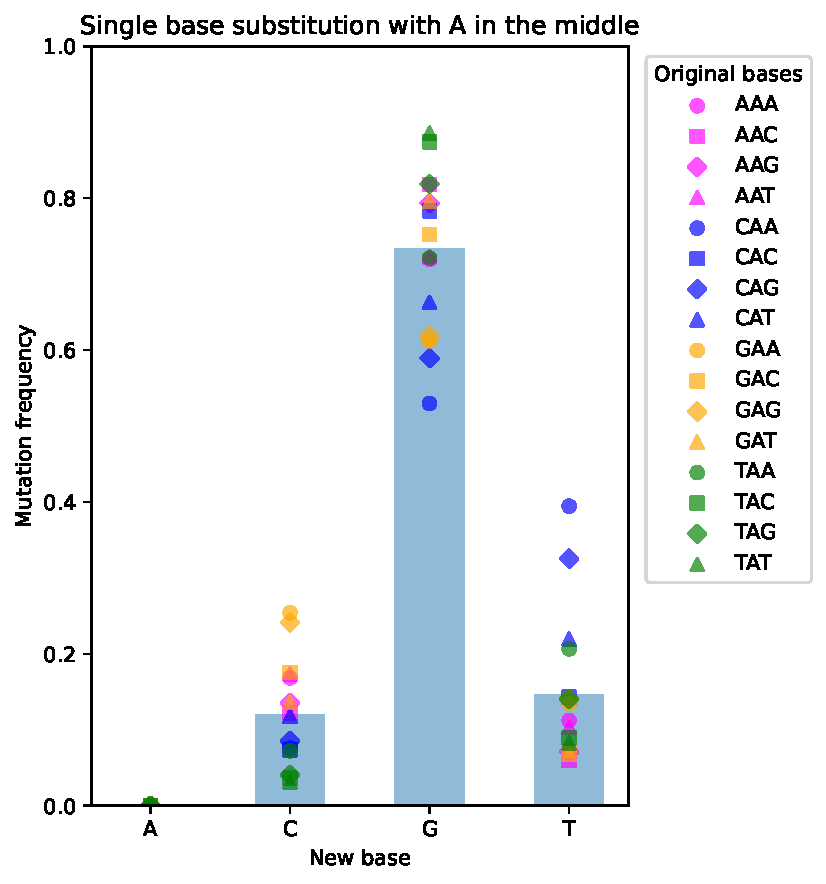
\includegraphics[width=0.45\linewidth]{fig_sbs_A.pdf}
    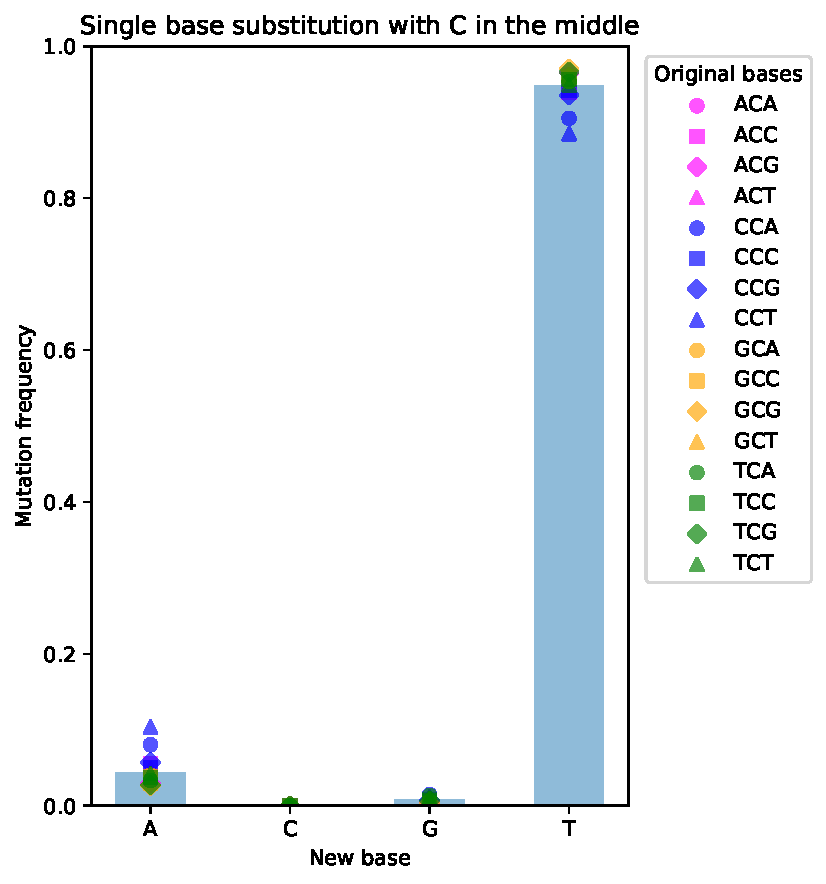
\includegraphics[width=0.45\linewidth]{fig_sbs_C.pdf}\\
    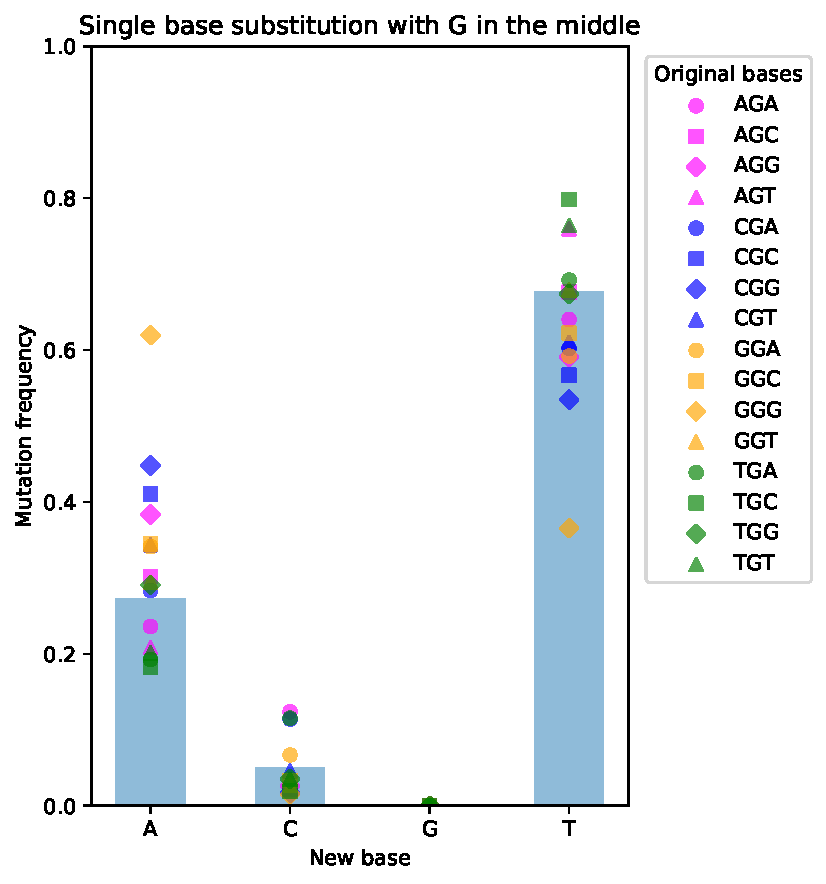
\includegraphics[width=0.45\linewidth]{fig_sbs_G.pdf}
    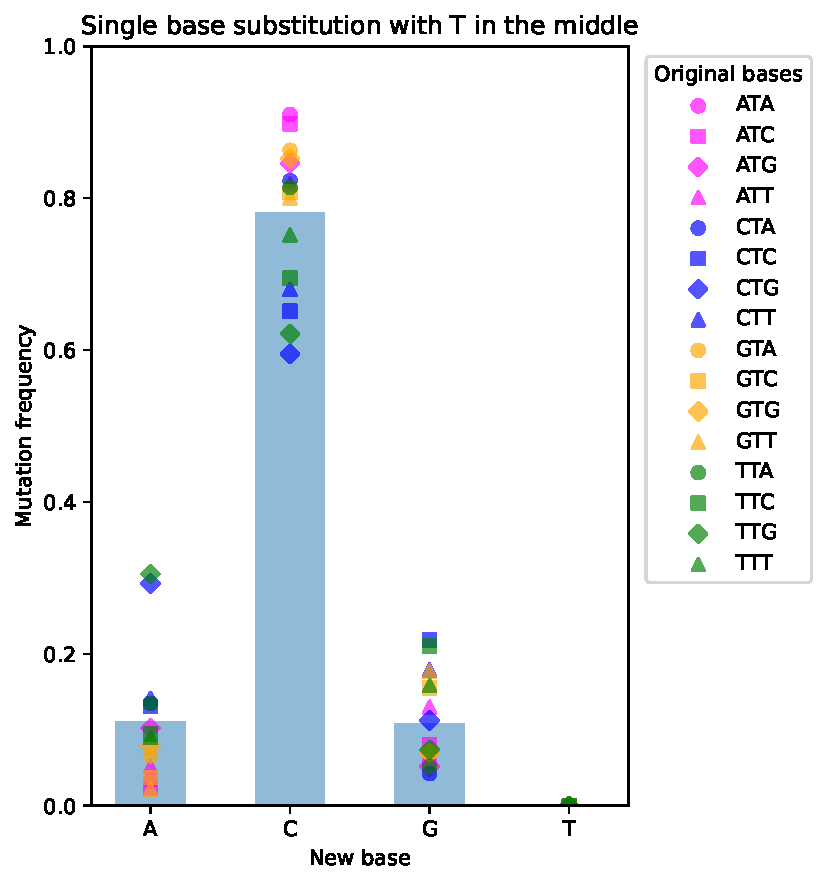
\includegraphics[width=0.45\linewidth]{fig_sbs_T.pdf}
    \caption{\textbf{Unconditional and context-conditioned substitution probabilities.}
    Bars show unconditional probabilities for each central-base substitution.
    Points show probabilities conditioned on the 16 possible trinucleotide
    contexts.}
    \label{fig:context-check}
\end{figure}

\section{CAC scoring and optimization}

\subsection{Score definition}

The main text defines CAC as a weighted mixture of standardized terms,
\begin{equation}
    S_{\rm CAC}
    =
    \alpha z(s_{\rm s})
    +\beta z(\log s_{\rm g})
    +\gamma z(\log p_T),
    \qquad
    \alpha,\beta,\gamma\geq0,\quad
    \alpha+\beta+\gamma=1.
    \label{eq:supp-cac}
\end{equation}
Here $s_{\rm s}$ is semantic change, $s_{\rm g}$ is grammaticality, and
$p_T$ is the codon-transition prior in Eq.~\eqref{eq:supp-aa-prob}. The
standardization $z(\cdot)$ is performed over all nonsynonymous single-nucleotide
substitutions of the reference Spike sequence.

\subsection{Validation sets}

Weights were optimized by minimizing the escape mean rank (EMR) on a specified
validation set. For a set $\mathcal{V}$ of known mutations,
\begin{equation}
    {\rm EMR}(\mathcal{V};\alpha,\beta,\gamma)
    =
    \frac{1}{|\mathcal{V}|}\sum_{m\in\mathcal{V}}
    {\rm rank}(m\mid\alpha,\beta,\gamma).
    \label{eq:supp-emr}
\end{equation}
The current results are retrospective benchmarks. A strict prospective deployment
should use time-split or leave-one-variant-out tuning to separate weight
selection from final testing.

\begin{table}[htbp]
    \centering
    \caption{\textbf{Validation sets used for retrospective optimization and evaluation.}}
    \begin{tabular}{l|p{0.72\textwidth}}
    \toprule
    \textbf{Name} & \textbf{Point mutations} \\
    \midrule
    DMS &
    \ttfamily K417E, K444Q, V445A, N450D, Y453F, L455F, E484K, G485D, F486V, F490L, F490S, Q493K, H655Y, R682Q, R685S, V687G, G769E, Q779K, V1128A \\
    \midrule
    Alpha &
    \ttfamily N501Y, A570D, D614G, P681H, T716I, S982A, D1118H \\
    \midrule
    Beta &
    \ttfamily L18F, D80A, D215G, K417N, E484K, N501Y, D614G, A701V \\
    \midrule
    Delta &
    \ttfamily T19R, G142D, L452R, T478K, D614G, P681R, D950N \\
    \midrule
    Omicron &
    \ttfamily A67V, T95I, G142D, L212I, G339D, S371L, S373P, S375F, K417N, N440K, G446S, S477N, T478K, E484A, Q493R, G496S, Q498R, N501Y, Y505H, T547K, D614G, H655Y, N679K, P681H, N764K, D796Y, N856K, Q954H, N969K, L981F \\
    \midrule
    Combined &
    \ttfamily A570D, A67V, A701V, D1118H, D215G, D614G, D796Y, D80A, D950N, E484A, E484K, F486V, F490L, F490S, G142D, G339D, G446S, G485D, G496S, G769E, H655Y, K417E, K417N, K444Q, L18F, L212I, L452R, L455F, L981F, N440K, N450D, N501Y, N679K, N764K, N856K, N969K, P681H, P681R, Q493K, Q493R, Q498R, Q779K, Q954H, R682Q, R685S, S371L, S373P, S375F, S477N, S982A, T19R, T478K, T547K, T716I, T95I, V1128A, V445A, V687G, Y453F, Y505H \\
    \bottomrule
    \end{tabular}
    \label{tab:validation-sets}
\end{table}

\subsection{Simplex search for optimal weights}

The rank transform makes EMR piecewise constant and non-differentiable. We
therefore used recursive subdivision of the simplex
$\Delta^2=\{(\alpha,\beta,\gamma):\alpha,\beta,\gamma\geq0,\alpha+\beta+\gamma=1\}$.
At each iteration the current triangle is divided into four subtriangles
(Fig.~\ref{fig:simplex-division}). For each subtriangle $T$ with vertices
$v_1,v_2,v_3$ and centroid $c$, we evaluate
\begin{equation}
    S(T)=\frac{1}{12}\left[
    {\rm EMR}(v_1)+{\rm EMR}(v_2)+{\rm EMR}(v_3)+9\,{\rm EMR}(c)
    \right],
\end{equation}
and continue with the subtriangle having the smallest $S(T)$.

\begin{figure}[htbp]
    \centering
    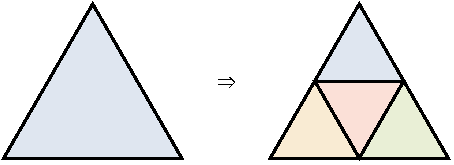
\includegraphics[width=0.35\linewidth]{supp_fig_division.pdf}
    \caption{\textbf{Recursive subdivision of the coefficient simplex.}}
    \label{fig:simplex-division}
\end{figure}

\section{Label-free calibration by phylogenetic fitness}

The main-text weights can be fixed without escape labels. We reparameterize the
score by freezing the codon-accessibility term at unit coefficient (an
\emph{offset}) and learning only the two protein-signal weights,
\begin{equation}
    S = b_0\, z(s_{\rm s}) + b_1\, z(\log s_{\rm g}) + \kappa\, z(\log p_T),
    \qquad \kappa = 1,
    \label{eq:supp-offset}
\end{equation}
and determine $(b_0,b_1)$ by logistic regression of the standardized protein
terms against a binarized \emph{phylogenetic-fitness} target, with the codon term
entering as a fixed offset. The target is the Bloom--Neher per-mutation fitness
$\Delta f = \ln[(n_{\rm actual}+P)/(n_{\rm expected}+P)]$, where expected counts
follow the neutral mutation spectrum at four-fold-degenerate third-codon-position
sites on the SARS-CoV-2 tree; $\Delta f$ is estimated from natural sequences
independently of the DMS escape benchmark. No escape label enters the fit.

Table~\ref{tab:supp-labelfree} compares the label-free weights and held-out DMS
escape AUROC against escape-supervised weights (obtained by fitting the same form
to DMS labels) across backbones. For the domain-adapted ESM-2$_{\rm cov}$ the
label-free weights $(0.285,0.942)$ recover the supervised weights $(0.268,0.955)$
and match its DMS AUROC; for general-purpose ESM-2, whose raw protein features
carry little escape signal, the fit correctly drives the protein weights toward
zero so that the score falls back on the mutation-process term without harm.

\begin{table}[htbp]
    \centering
    \caption{\textbf{Label-free vs escape-supervised calibration across backbones.}
    Weights $(b_0,b_1)$ on semantic change and grammaticality (codon prior frozen,
    $\kappa=1$); DMS escape AUROC. ``bloom-fit'' is fit to phylogenetic fitness
    (no escape labels); ``supervised'' is fit to DMS labels (reference).}
    \begin{tabular}{l|l|cc|c}
        \toprule
        Backbone & Method & $b_0$ (sem.) & $b_1$ (gram.) & DMS AUROC \\
        \midrule
        base ESM-2 & equal $(1,1)$      & $1.000$  & $1.000$  & $0.786$ \\
                   & CLIB-only          & $0.000$  & $0.000$  & $0.883$ \\
                   & bloom-fit          & $-0.102$ & $0.449$  & $0.863$ \\
                   & supervised (DMS)   & $0.094$  & $0.313$  & $0.880$ \\
        \midrule
        ESM-2$_{\rm cov}$ & equal $(1,1)$    & $1.000$ & $1.000$ & $0.884$ \\
                          & CLIB-only        & $0.000$ & $0.000$ & $0.883$ \\
                          & \textbf{bloom-fit} & $\mathbf{0.285}$ & $\mathbf{0.942}$ & $\mathbf{0.899}$ \\
                          & supervised (DMS) & $0.268$ & $0.955$ & $0.898$ \\
        \bottomrule
    \end{tabular}
    \label{tab:supp-labelfree}
\end{table}

Three independent evolutionary signals yield concordant weights on
ESM-2$_{\rm cov}$ (Table~\ref{tab:supp-crosssignal}): all-time substitution
frequency, phylogenetic fitness, and an early-period ($\le$2021) temporal split.
All favor grammaticality over semantic change and reproduce the supervised
operating point, indicating that the calibration is a property of the mutation
process rather than of any single proxy.

\begin{table}[htbp]
    \centering
    \caption{\textbf{Cross-signal convergence of label-free weights (ESM-2$_{\rm cov}$).}}
    \begin{tabular}{l|cc|c}
        \toprule
        Fitting signal & $b_0$ (sem.) & $b_1$ (gram.) & DMS AUROC \\
        \midrule
        Frequency (all-time)    & $0.191$ & $1.543$ & $0.883$ \\
        Phylogenetic fitness    & $0.285$ & $0.942$ & $0.899$ \\
        Temporal (early split)  & $0.194$ & $1.681$ & $0.881$ \\
        \bottomrule
    \end{tabular}
    \label{tab:supp-crosssignal}
\end{table}

\section{Prospective and leave-one-variant-out validation}

A calibration without escape labels can be made strictly prospective. We fit
$(b_0,b_1)$ on substitution frequencies observed before a date cutoff and evaluate
on substitutions that rose in frequency afterward. Because the PLM terms are
frequency-independent and the future is unavailable at fit time, this is a genuine
held-out forecast. Table~\ref{tab:supp-temporal} reports the emergence-forecast
AUROC at three cutoffs, with paired-bootstrap $95\%$ confidence intervals for the
improvement over an equal-weight baseline. The label-free score forecasts emergent
substitutions up to AUROC $0.90$, significantly above equal weight at the two
earlier cutoffs and comparable to the escape-supervised reference ($0.894$), which
it never sees.

\begin{table}[htbp]
    \centering
    \caption{\textbf{Prospective emergence forecasting.} Weights fit on pre-cutoff
    frequency; evaluated on post-cutoff emergent substitutions. $\Delta$AUROC is
    label-free minus equal-weight, with paired-bootstrap $95\%$ CI.}
    \begin{tabular}{l|c|ccc|c}
        \toprule
        Cutoff & $n_{\rm emg}$ & equal & CLIB-only & label-free & $\Delta$AUROC (95\% CI) \\
        \midrule
        2021-06 & 25 & $0.940$ & $0.885$ & $0.976$ & $+0.036\;[0.025,\,0.046]$ \\
        2021-12 & 15 & $0.860$ & $0.836$ & $0.899$ & $+0.038\;[0.017,\,0.061]$ \\
        2022-06 & 34 & $0.807$ & $0.838$ & $0.824$ & $+0.018\;[-0.003,\,0.038]$ \\
        \bottomrule
    \end{tabular}
    \label{tab:supp-temporal}
\end{table}

To confirm that the improvement is not memorization of the evaluated annotations,
we recalibrated with leave-one-variant-out: for each lineage, its defining
substitutions were removed from the fitting set before weights were determined and
the lineage was then scored. The gain over equal weight persisted on all tested
lineages (each $95\%$ bootstrap CI on the AUROC improvement excluded zero for
lineages with $\ge 7$ positives), so the calibration generalizes to substitutions
it never used.

\section{Model backbones and computational environment}

We evaluated four PLM backbones: the viral Hie-BiLSTM model \cite{hie2021learning}
and ESM-2-150M, ESM-2-650M, and ESM-2-3B \cite{lin2023evolutionary}. For
Hie-BiLSTM, we used precomputed semantic and grammaticality scores from the
original authors. ESM-2 scores were generated on a server with a single NVIDIA
H100 80GB GPU, two AMD EPYC 9124 16-core CPUs, and 768GB RAM, running Ubuntu
24.04.2 LTS. The Python environment used Python 3.10.17, PyTorch 2.7.0,
Transformers 4.51.3, and CUDA 12.8.

\begin{figure}[htbp]
    \centering
    \begin{tabular}{@{}cc@{}}
        \small ESM-2-150M & \small ESM-2-650M \\
        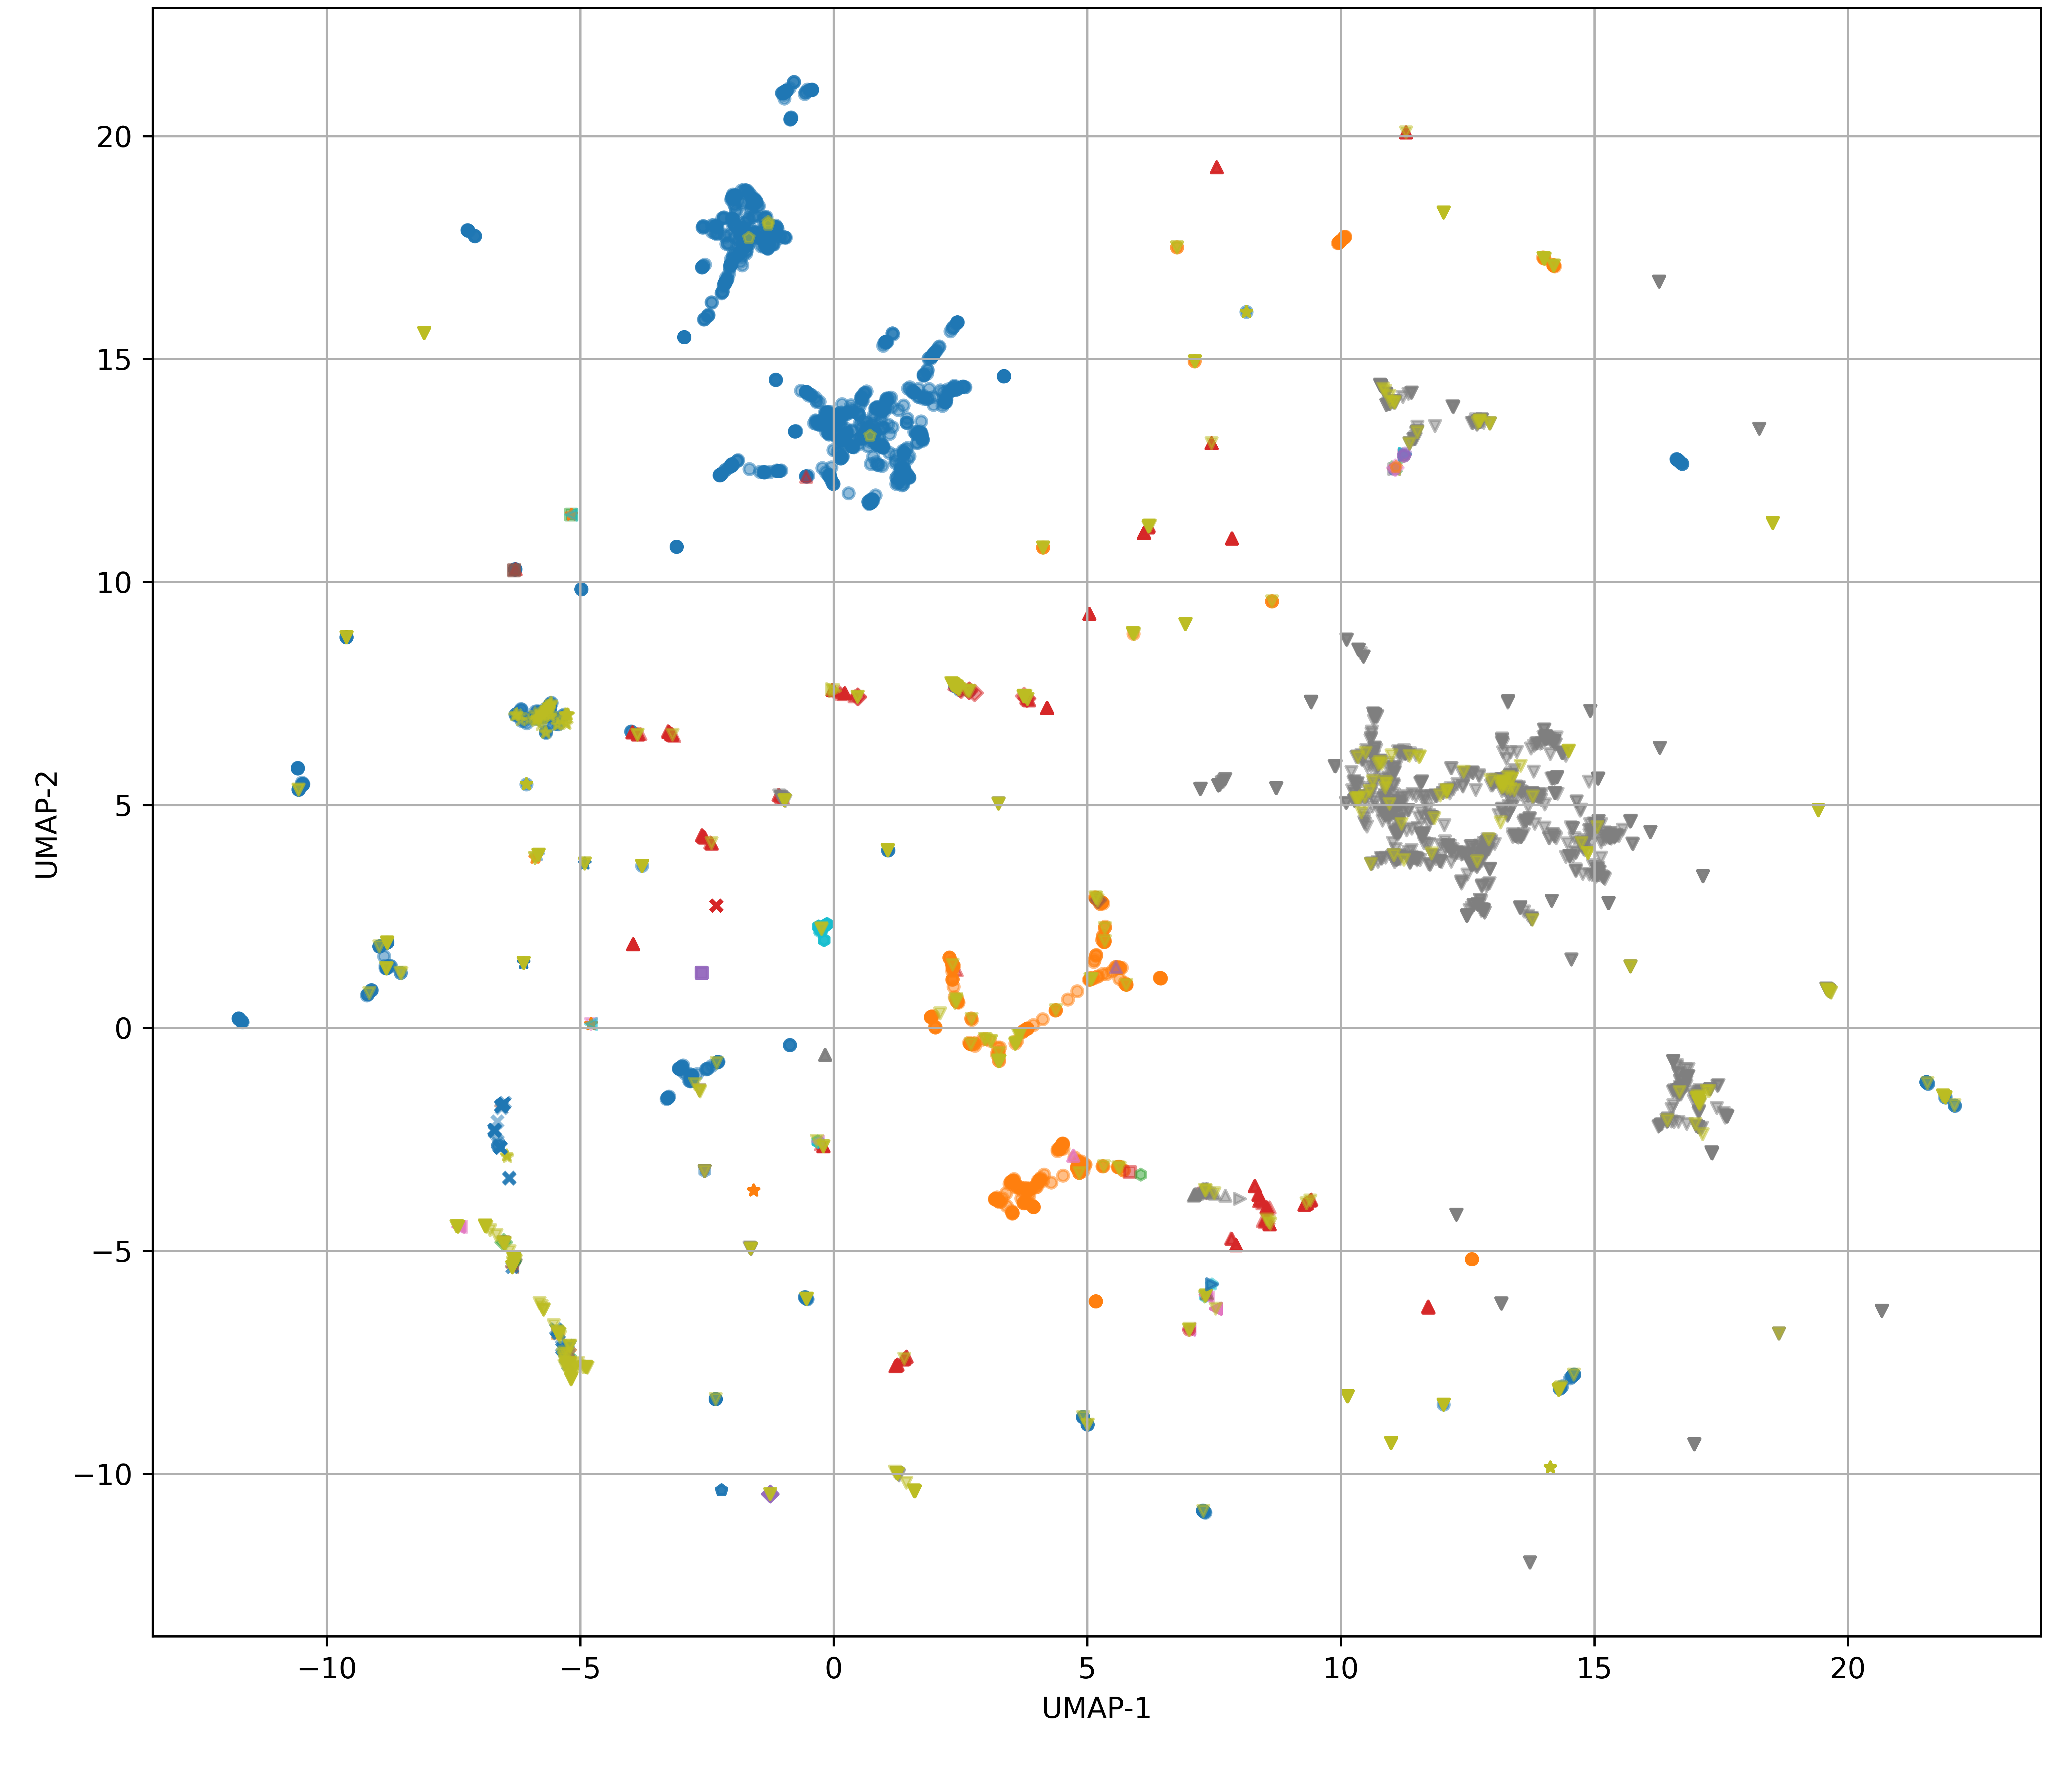
\includegraphics[width=0.48\linewidth]{fig_umap_projection_150M.png}
        & 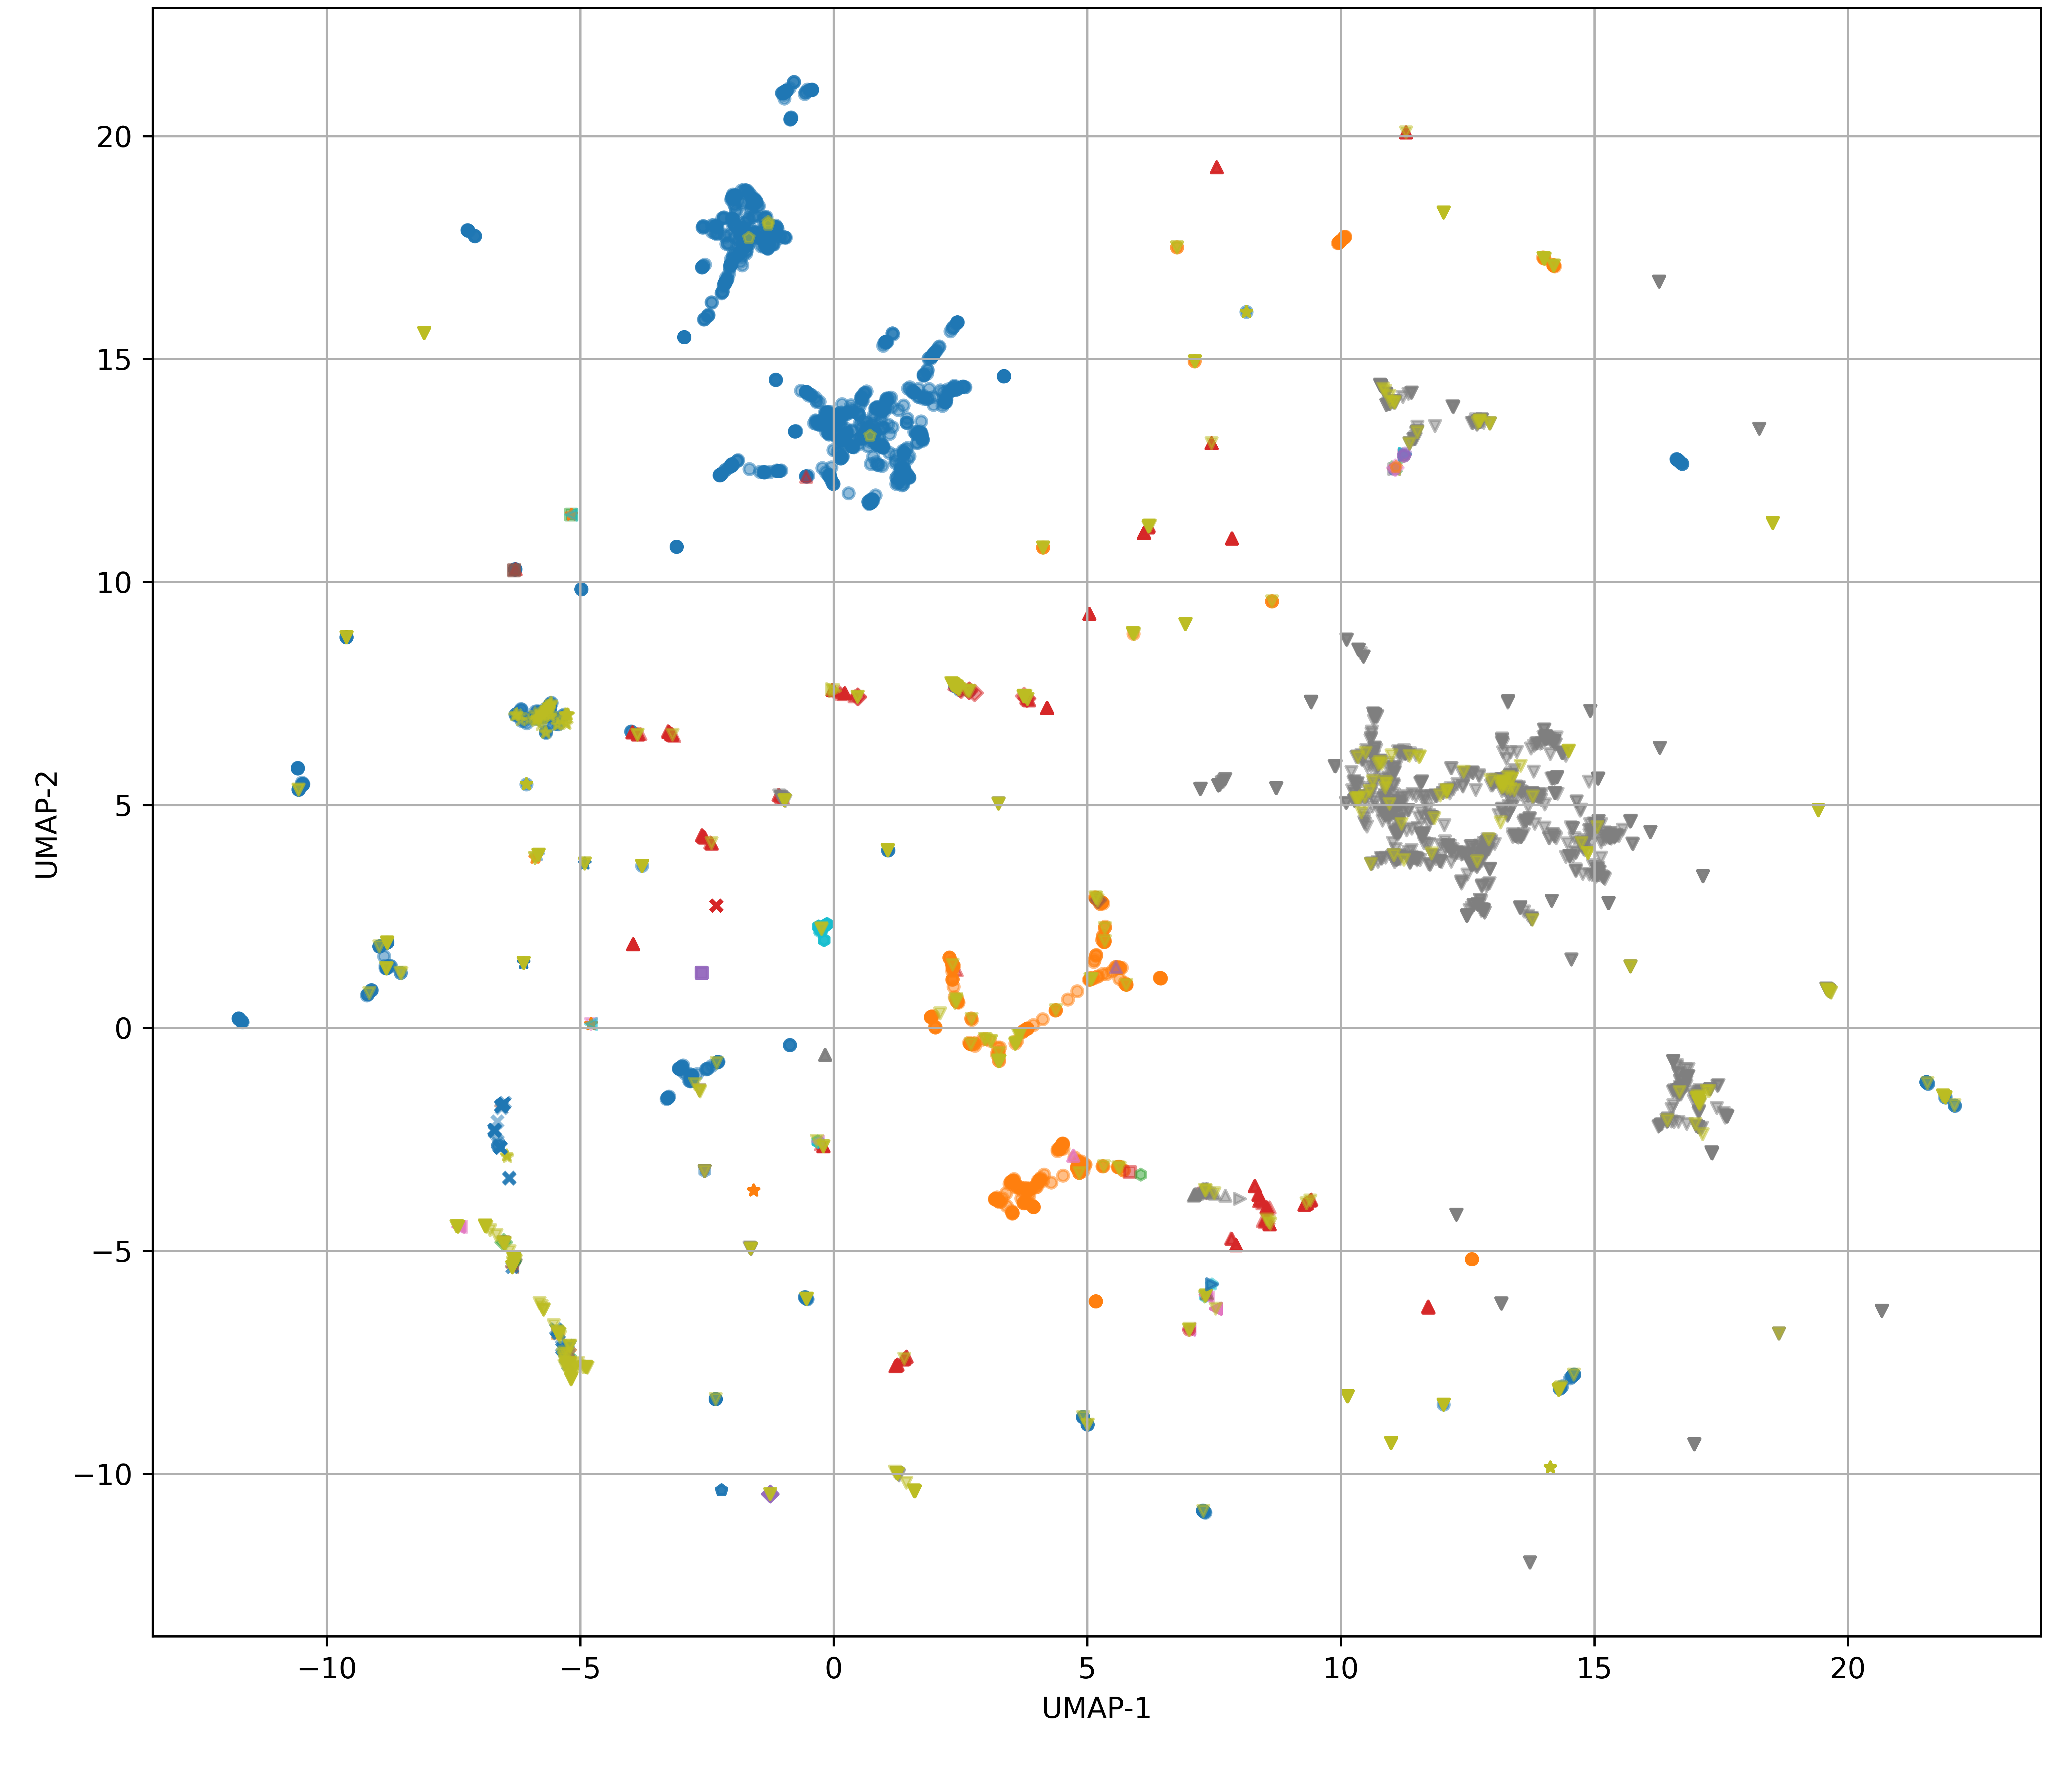
\includegraphics[width=0.48\linewidth]{fig_umap_projection_650M.png} \\
        \small ESM-2-3B & \\
        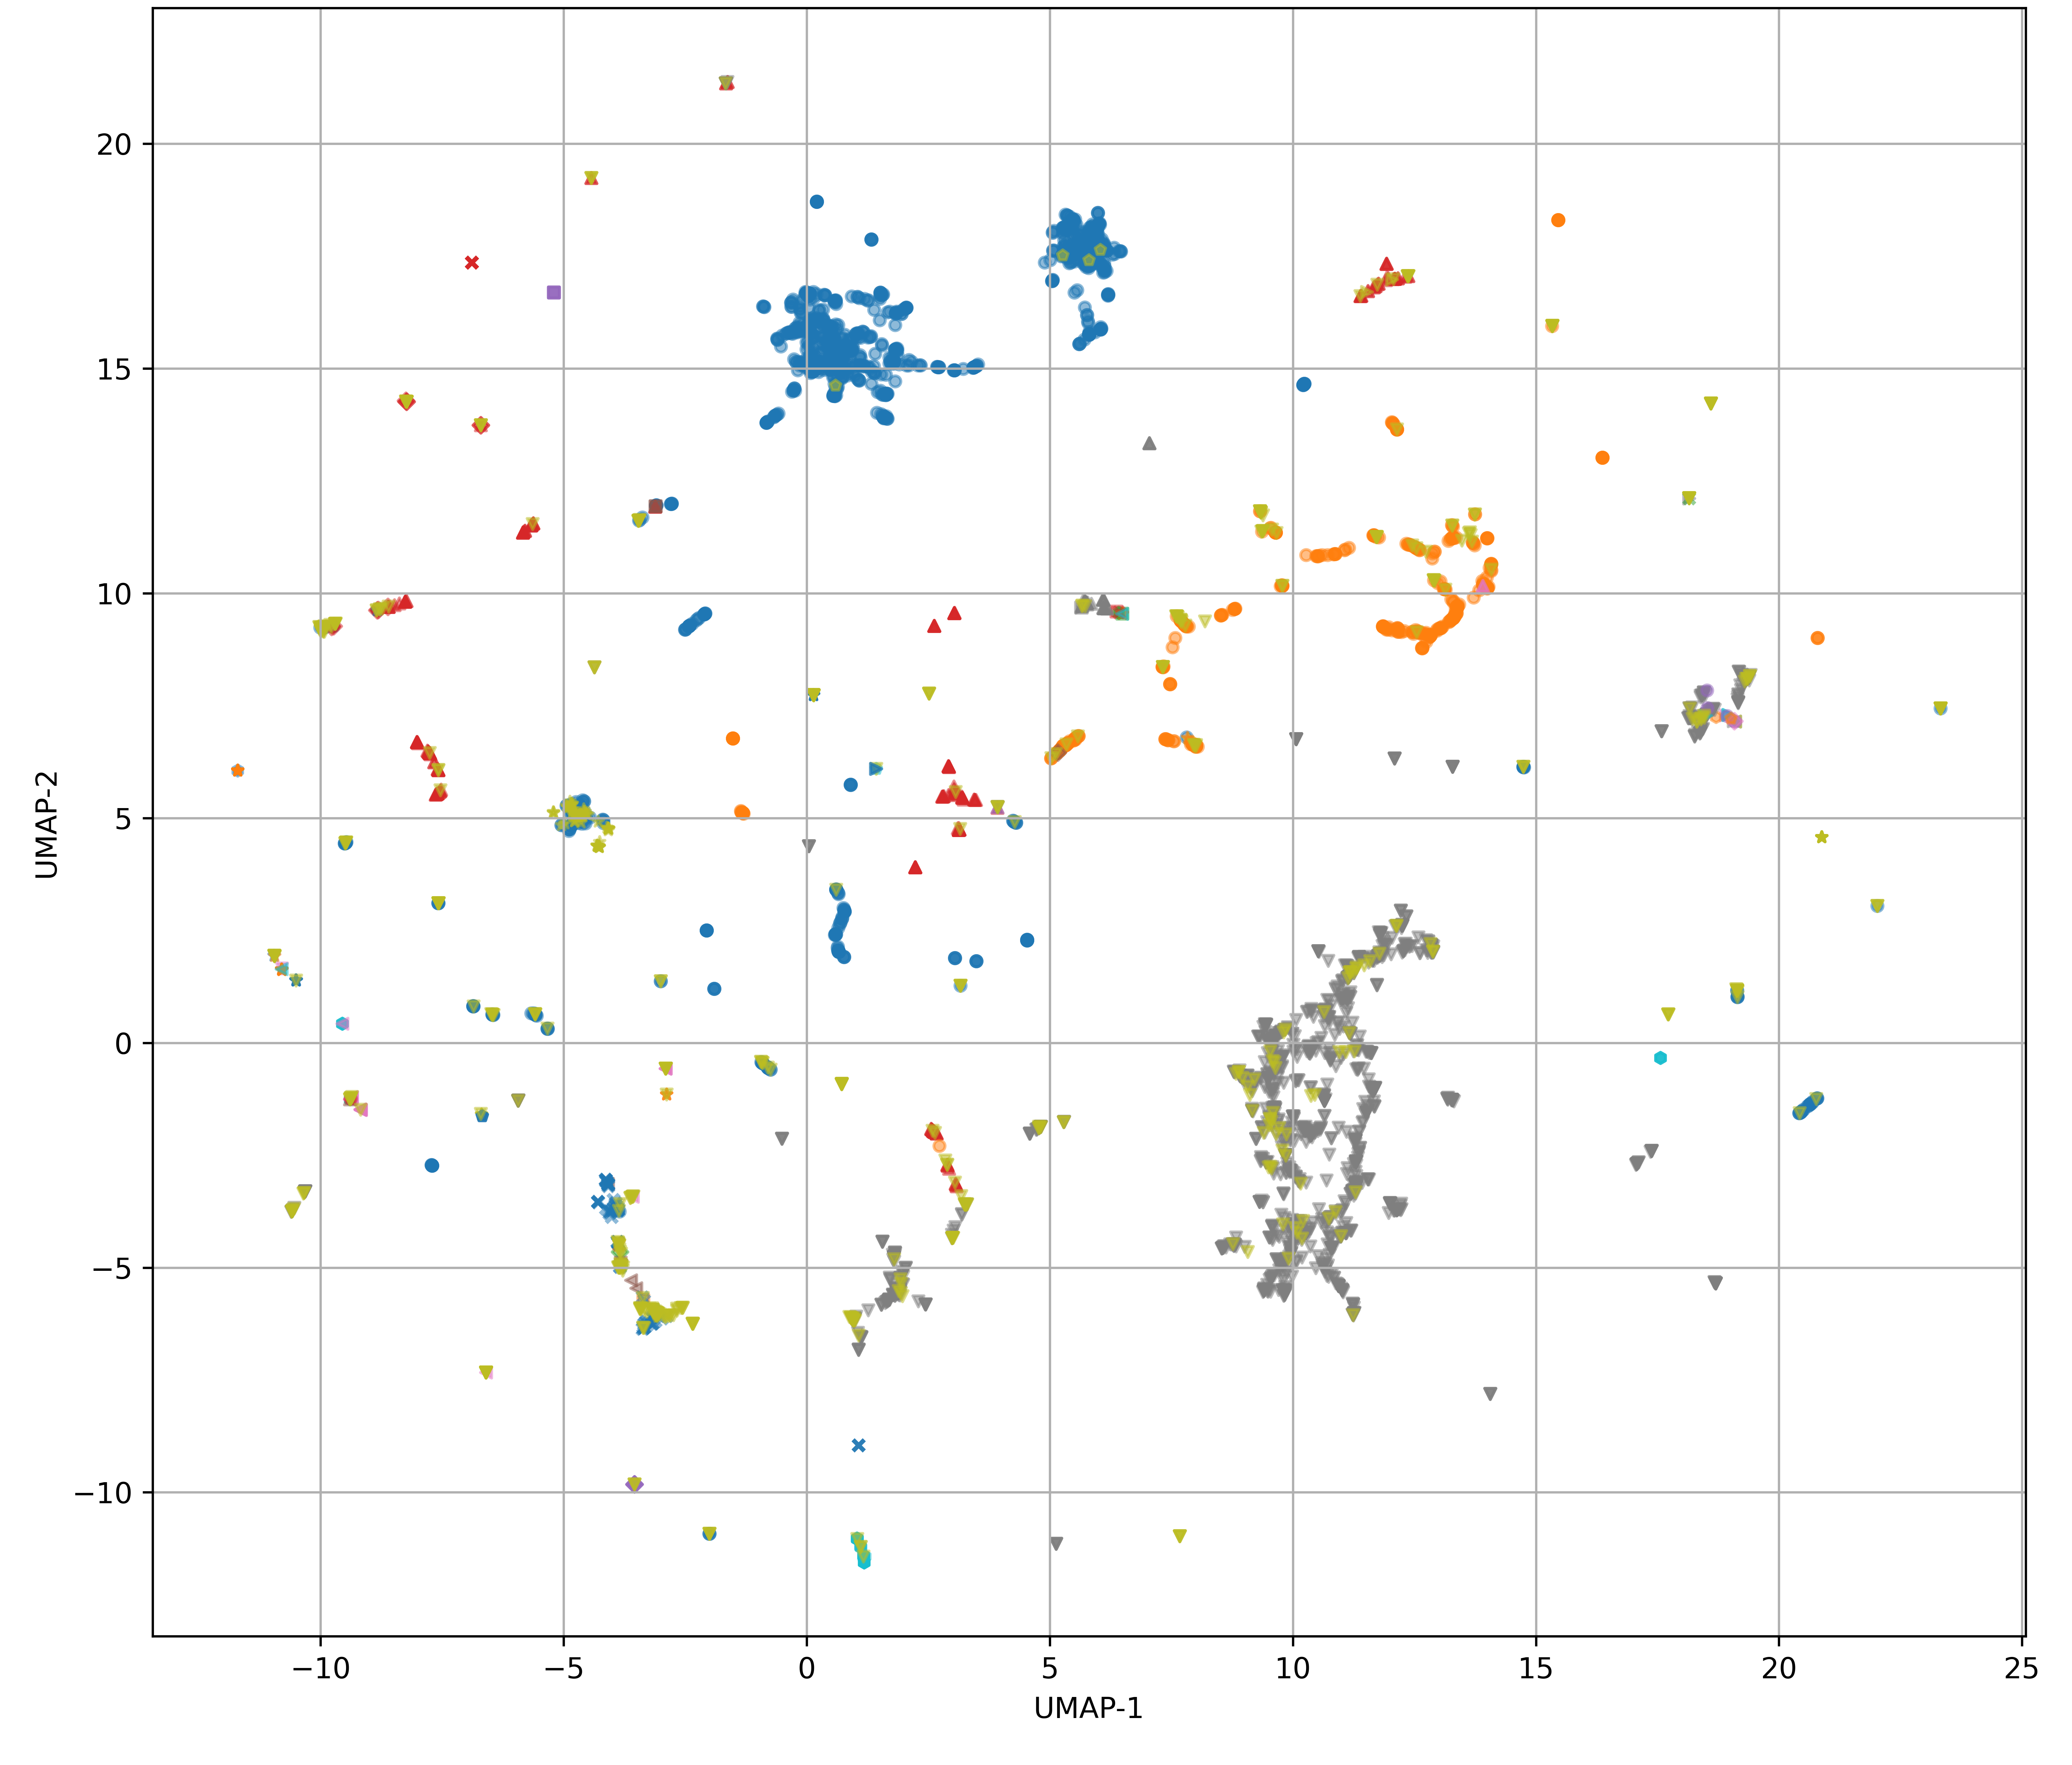
\includegraphics[width=0.48\linewidth]{fig_umap_projection_3B.png}
        & \raisebox{0.5\height}{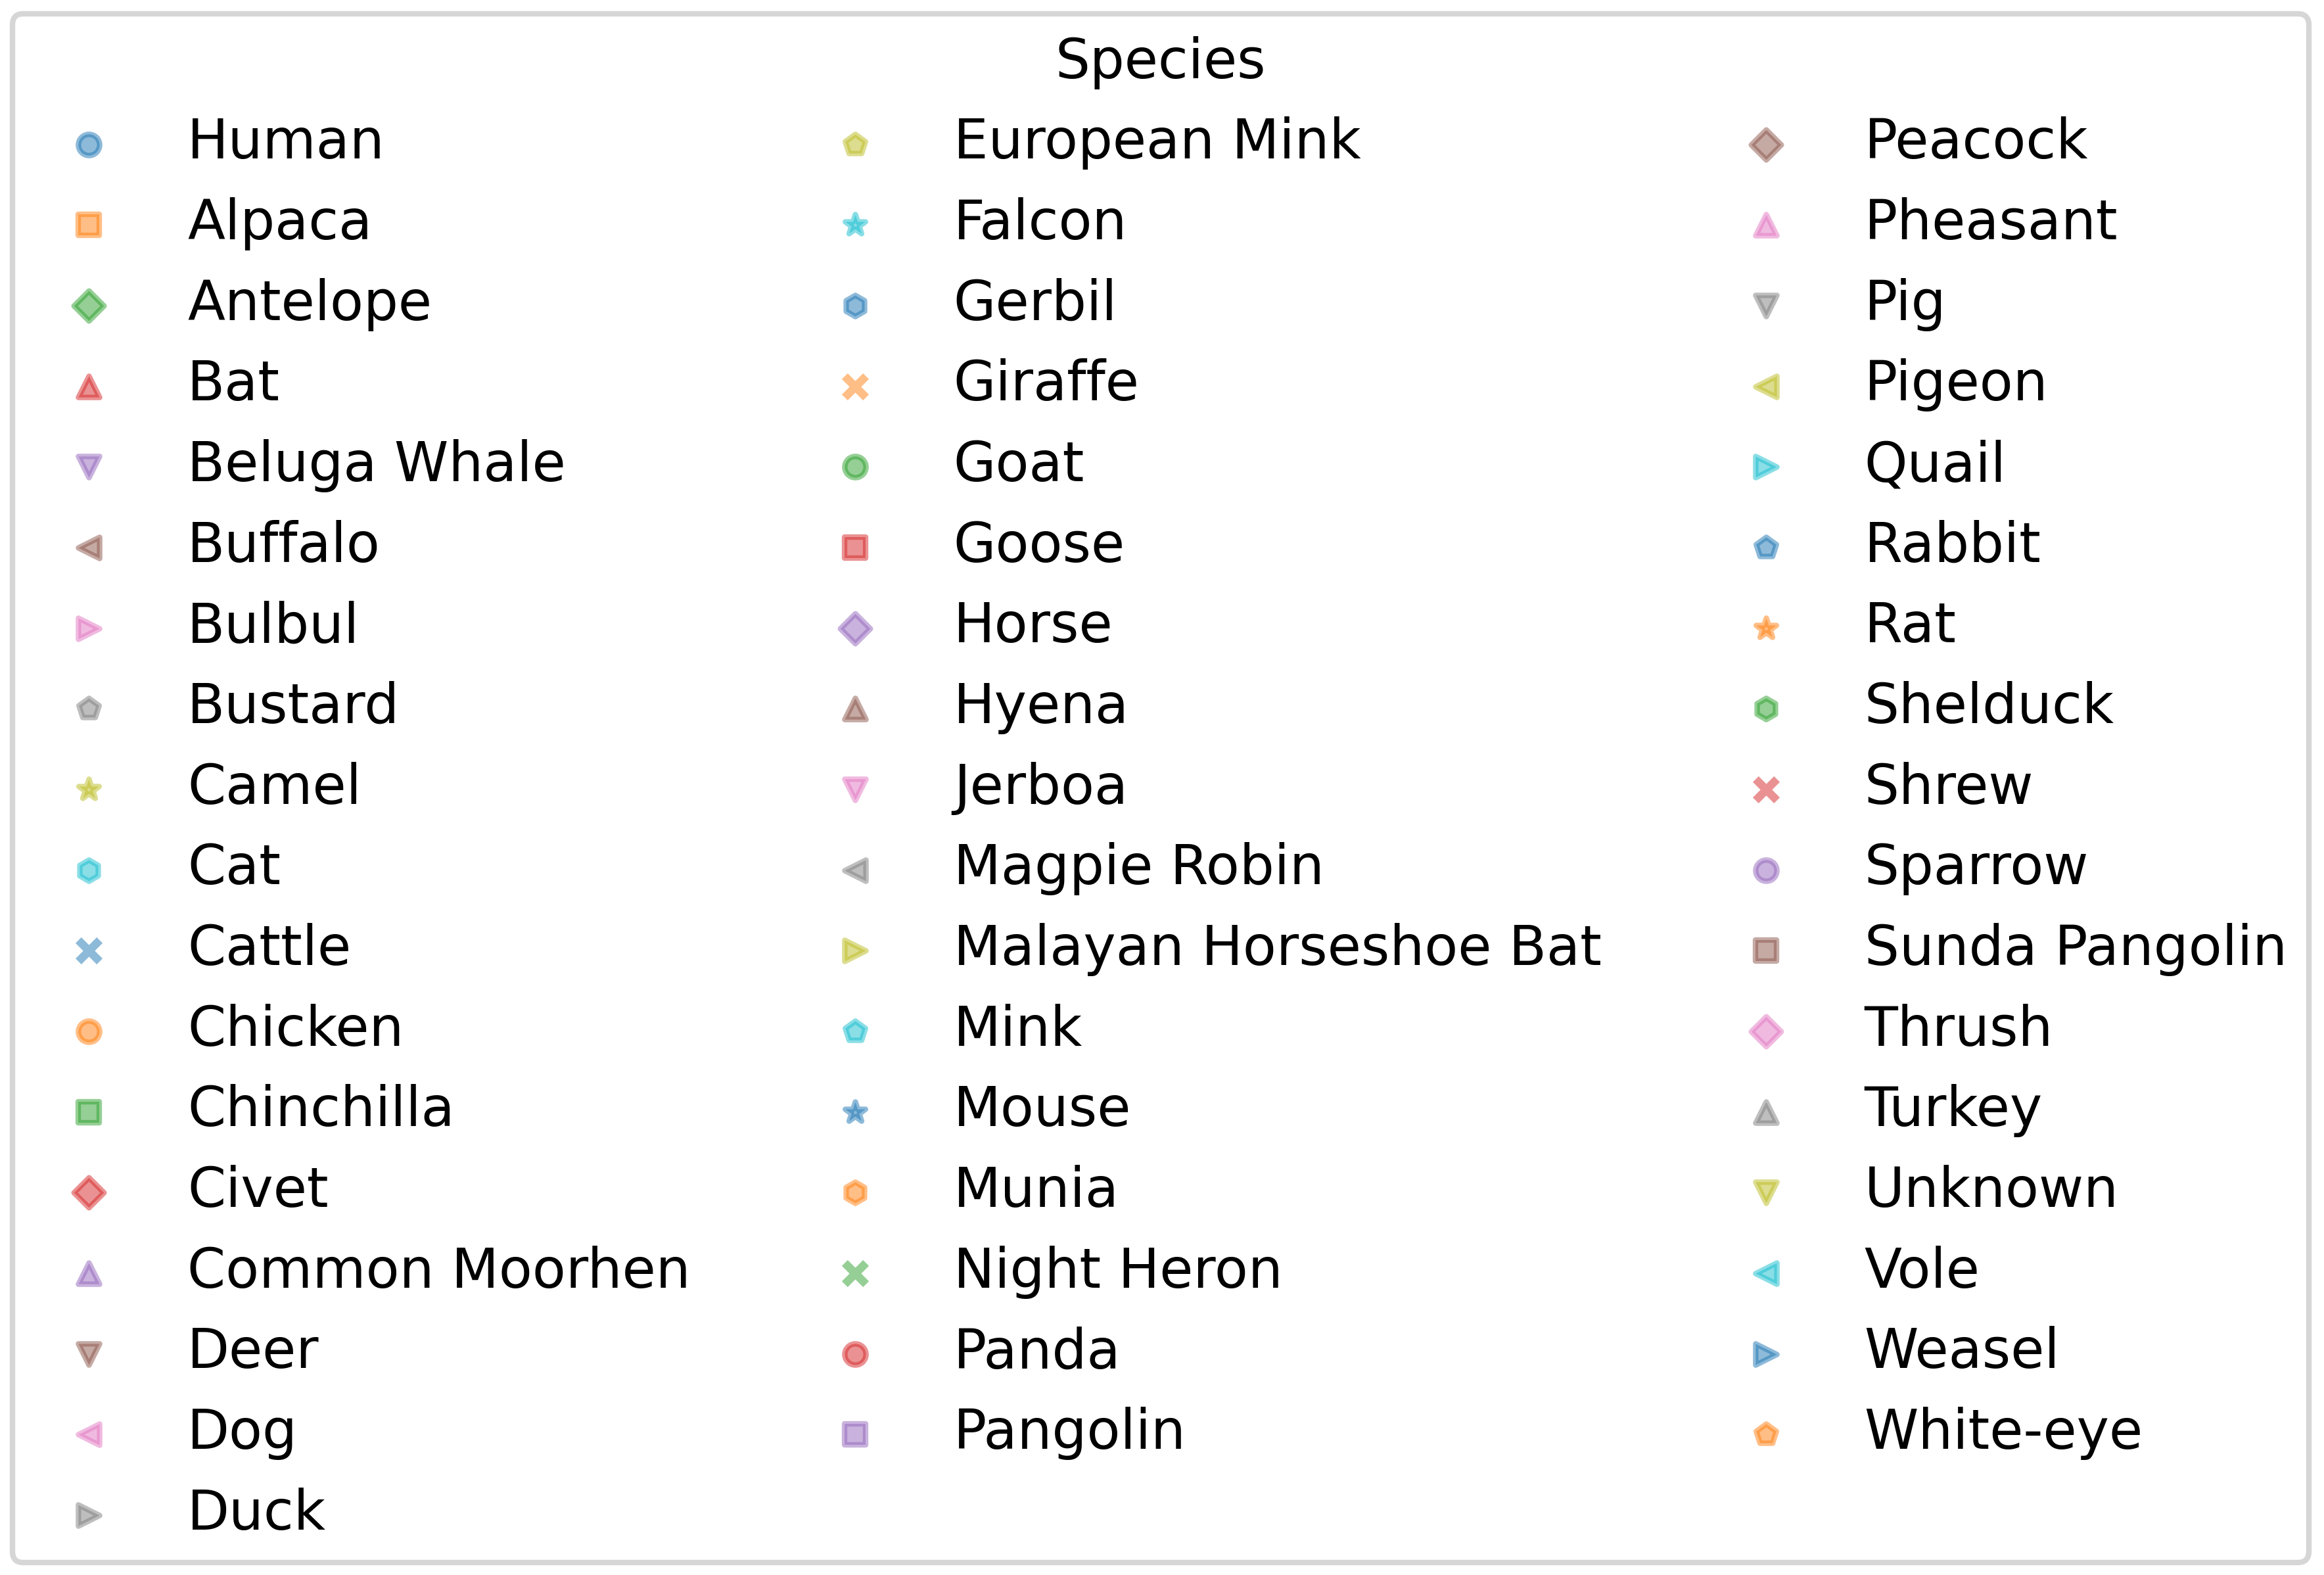
\includegraphics[width=0.30\linewidth]{fig_umap_projection_legend.png}}
    \end{tabular}
    \caption{\textbf{UMAP projections of ESM-2 Spike embeddings.}
    Points represent unique SARS-CoV-2 Spike sequences colored by host species.}
    \label{fig:umap}
\end{figure}

\section{Additional performance results}

\begin{table}[htbp]
    \centering
    \caption{\textbf{Comprehensive mean-rank comparison of CSCS and CAC.}}
    \begin{tabular}{c|c|c|c|c}
        \toprule
        \multirow{2}{*}{\makecell{\textbf{Validation}\\\textbf{set}}}
        & \multirow{2}{*}{\makecell{\textbf{Model}\\\textbf{backbone}}}
        & \multicolumn{2}{c|}{\textbf{Escape rank (mean $\pm$ s.d.)}}
        & \multirow{2}{*}{\makecell{\textbf{Wilcoxon}\\\textbf{$p$-value}}} \\
        \cmidrule{3-4}
        & & \textbf{CSCS} & \textbf{CAC} & \\
        \midrule
        DMS & Hie-BiLSTM & 3757.16 $\pm$ 2573.64 & 3493.47 $\pm$ 2973.51 & $0.55$ \\
        DMS & ESM-2-150M & 9387.26 $\pm$ 6127.43 & 5098.11 $\pm$ 3667.28 & $6.2\times10^{-3}$ \\
        DMS & ESM-2-650M & 8562.32 $\pm$ 6869.83 & 5143.42 $\pm$ 3701.19 & $1.3\times10^{-2}$ \\
        DMS & ESM-2-3B & 9130.00 $\pm$ 6500.32 & 5037.16 $\pm$ 3586.46 & $3.1\times10^{-3}$ \\
        \midrule
        Alpha & Hie-BiLSTM & 7032.43 $\pm$ 5084.98 & 3567.86 $\pm$ 3281.72 & $0.11$ \\
        Alpha & ESM-2-150M & 10427.86 $\pm$ 6253.14 & 6732.86 $\pm$ 4672.34 & $0.19$ \\
        Alpha & ESM-2-650M & 12948.43 $\pm$ 5753.63 & 6816.29 $\pm$ 4391.33 & $0.11$ \\
        Alpha & ESM-2-3B & 10766.14 $\pm$ 5597.26 & 6480.71 $\pm$ 4743.41 & $0.11$ \\
        \midrule
        Beta & Hie-BiLSTM & 4046.00 $\pm$ 2348.84 & 1339.75 $\pm$ 1893.99 & $2.7\times10^{-2}$ \\
        Beta & ESM-2-150M & 7902.00 $\pm$ 5731.57 & 3545.25 $\pm$ 3618.94 & $7.8\times10^{-3}$ \\
        Beta & ESM-2-650M & 7932.25 $\pm$ 4493.72 & 3368.38 $\pm$ 3302.71 & $2.0\times10^{-2}$ \\
        Beta & ESM-2-3B & 5013.25 $\pm$ 2767.09 & 2697.88 $\pm$ 2765.35 & $2.7\times10^{-2}$ \\
        \midrule
        Delta & Hie-BiLSTM & 8102.29 $\pm$ 7945.03 & 5107.57 $\pm$ 7242.10 & $0.15$ \\
        Delta & ESM-2-150M & 11119.86 $\pm$ 5348.50 & 7255.43 $\pm$ 4137.39 & $7.8\times10^{-3}$ \\
        Delta & ESM-2-650M & 11190.29 $\pm$ 5828.41 & 7094.71 $\pm$ 3428.05 & $3.9\times10^{-2}$ \\
        Delta & ESM-2-3B & 10644.57 $\pm$ 4260.09 & 6154.71 $\pm$ 2643.14 & $2.3\times10^{-2}$ \\
        \midrule
        Omicron & Hie-BiLSTM & 7655.30 $\pm$ 5208.90 & 3258.77 $\pm$ 3557.71 & $7.0\times10^{-6}$ \\
        Omicron & ESM-2-150M & 10366.23 $\pm$ 5749.98 & 4261.67 $\pm$ 3283.74 & $7.0\times10^{-6}$ \\
        Omicron & ESM-2-650M & 8687.47 $\pm$ 5740.13 & 4140.77 $\pm$ 3198.91 & $1.5\times10^{-5}$ \\
        Omicron & ESM-2-3B & 8680.50 $\pm$ 6125.22 & 4059.87 $\pm$ 3336.31 & $8.5\times10^{-5}$ \\
        \midrule
        Combined & Hie-BiLSTM & 6259.70 $\pm$ 5377.95 & 3841.07 $\pm$ 4183.94 & $2.4\times10^{-4}$ \\
        Combined & ESM-2-150M & 9815.72 $\pm$ 6052.50 & 5308.55 $\pm$ 4280.29 & $1.3\times10^{-6}$ \\
        Combined & ESM-2-650M & 8857.37 $\pm$ 6263.02 & 5326.83 $\pm$ 4195.95 & $1.6\times10^{-5}$ \\
        Combined & ESM-2-3B & 8735.83 $\pm$ 6094.85 & 5204.23 $\pm$ 4054.37 & $8.6\times10^{-6}$ \\
        \bottomrule
    \end{tabular}
    \label{tab:all-performance}
\end{table}

\begin{figure}[htbp]
    \centering
    \begin{tabular}{@{}cc@{}}
    \small Alpha & \small Beta \\
    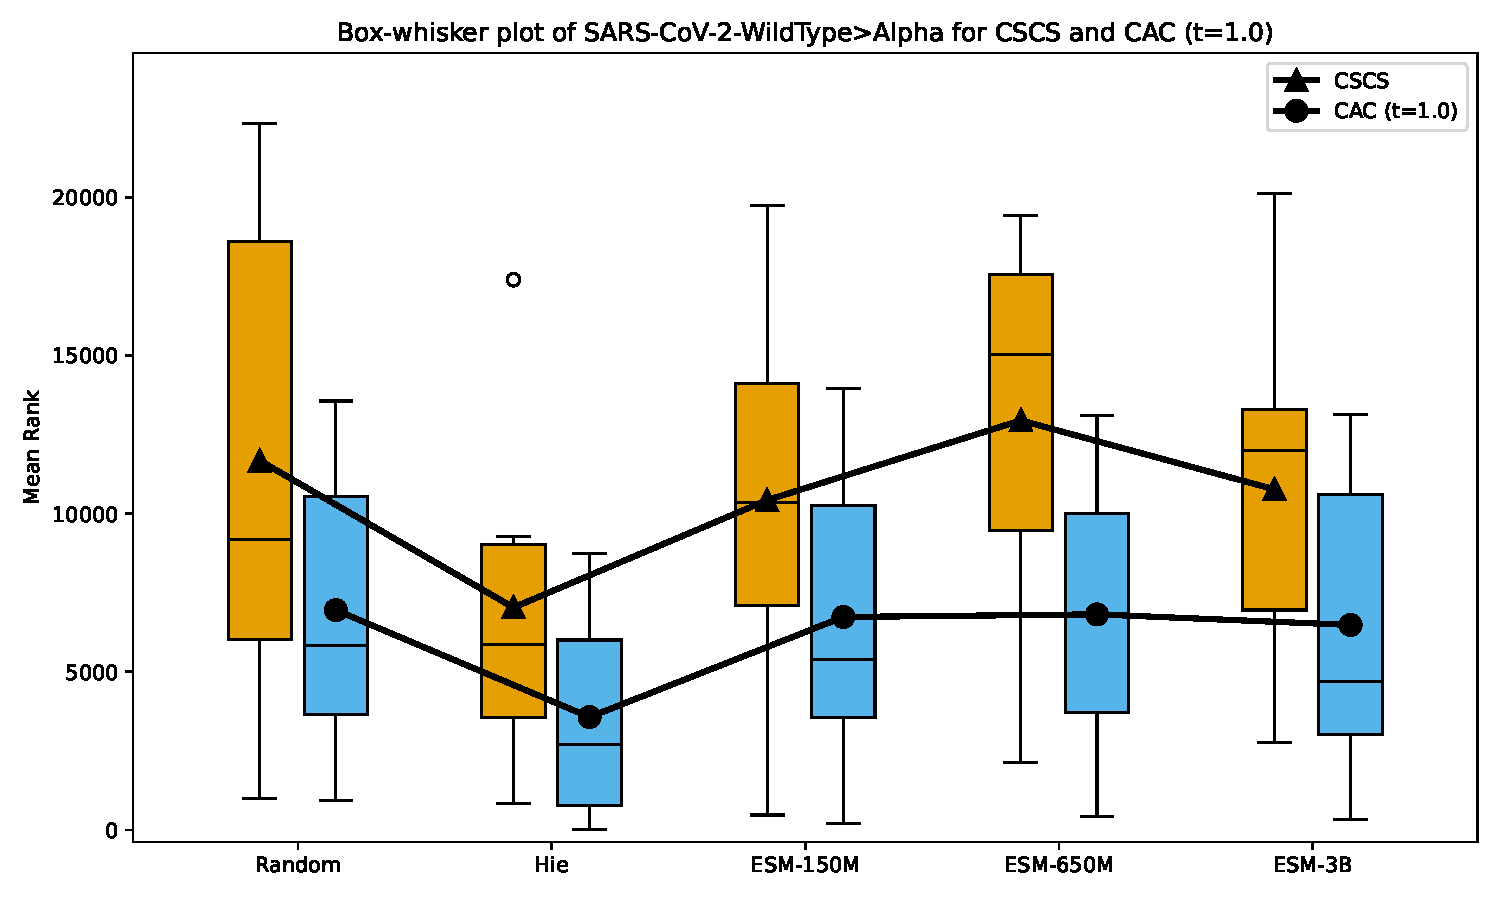
\includegraphics[width=0.48\linewidth]{boxplot-(e=wt2alpha)-(t=1.0).pdf} &
    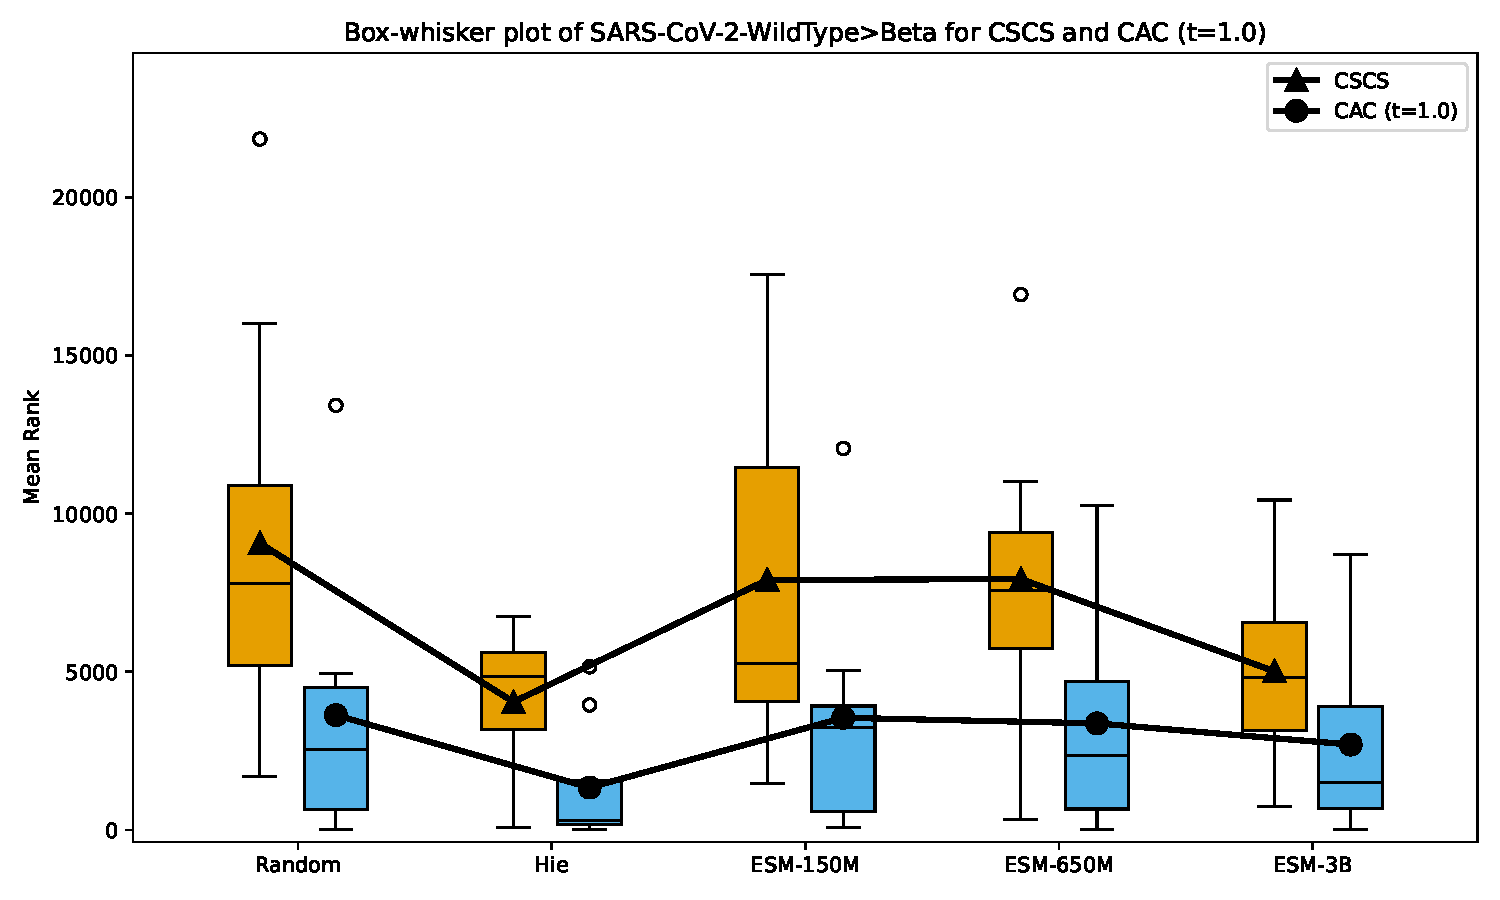
\includegraphics[width=0.48\linewidth]{boxplot-(e=wt2beta)-(t=1.0).pdf} \\
    \small Delta & \small Omicron \\
    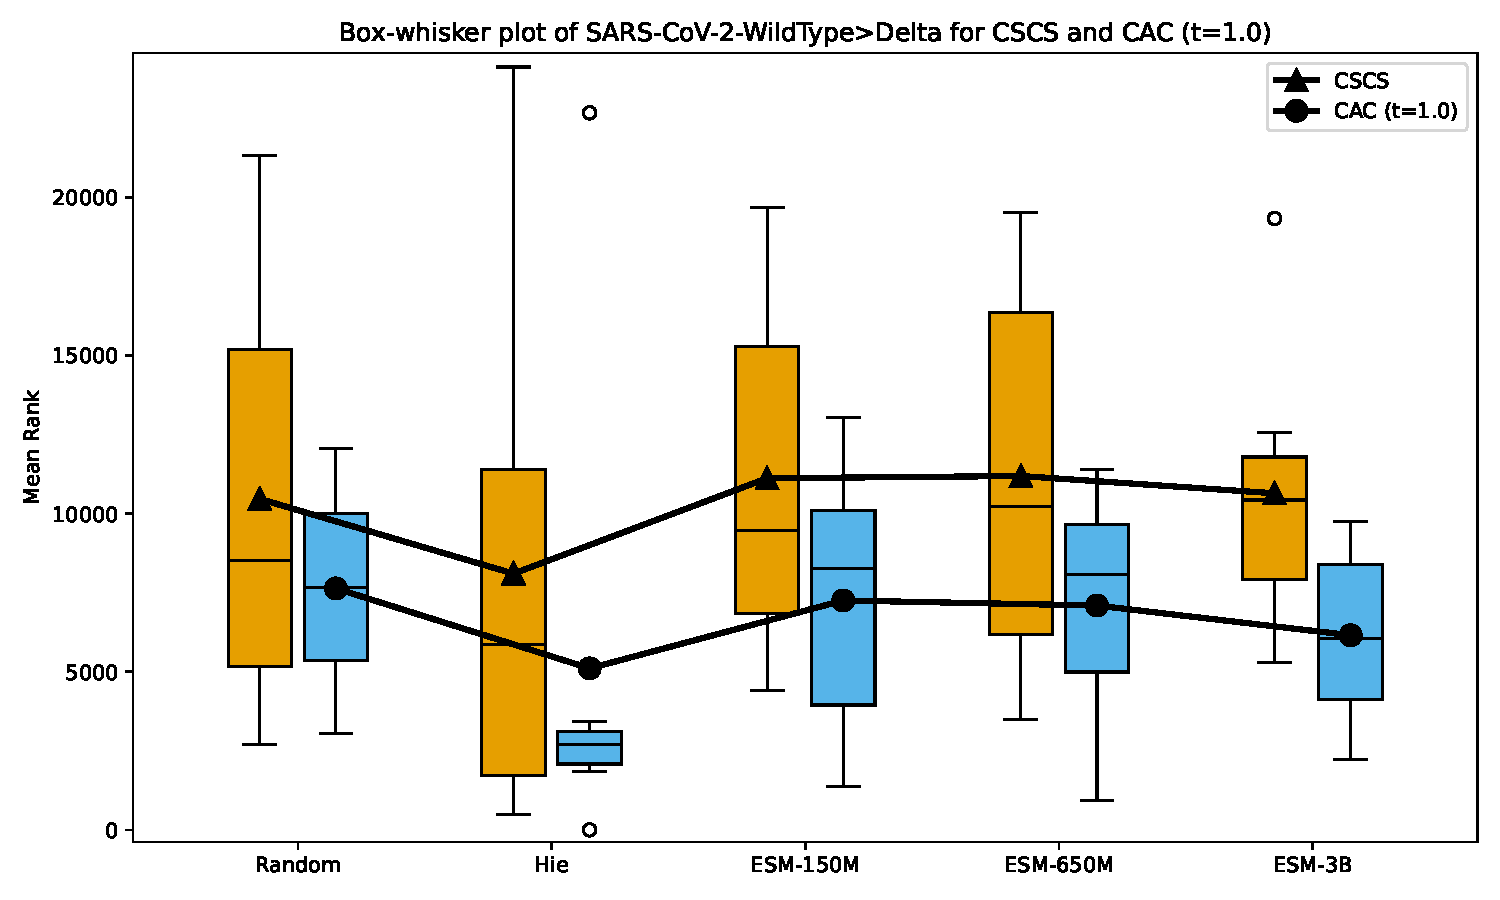
\includegraphics[width=0.48\linewidth]{boxplot-(e=wt2delta)-(t=1.0).pdf} &
    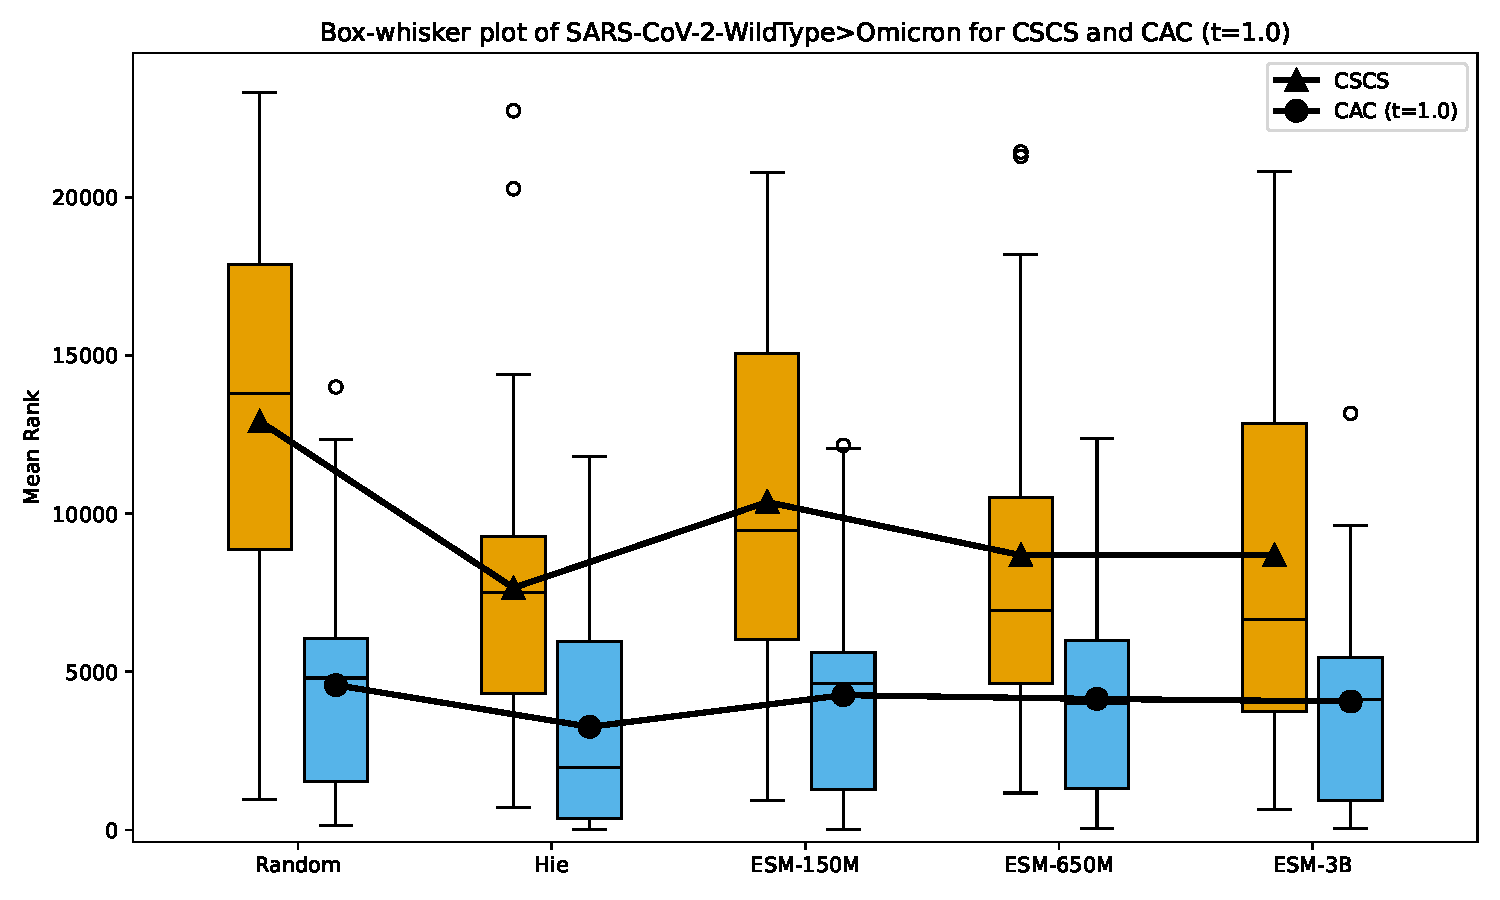
\includegraphics[width=0.48\linewidth]{boxplot-(e=wt2omicron)-(t=1.0).pdf} \\
    \small DMS & \small Combined \\
    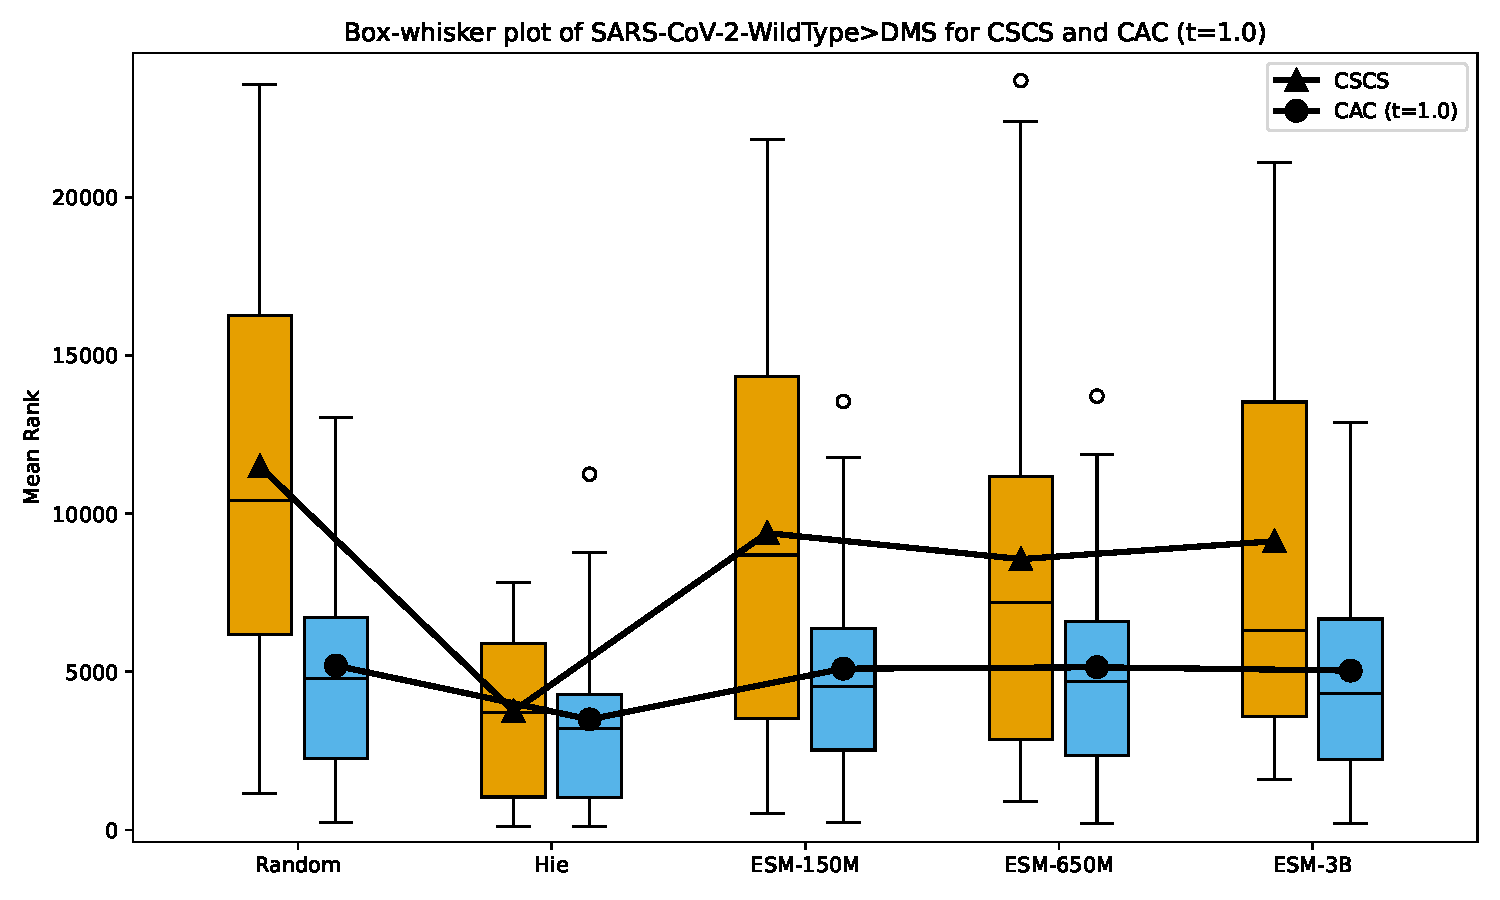
\includegraphics[width=0.48\linewidth]{boxplot-(e=wt2dms)-(t=1.0).pdf} &
    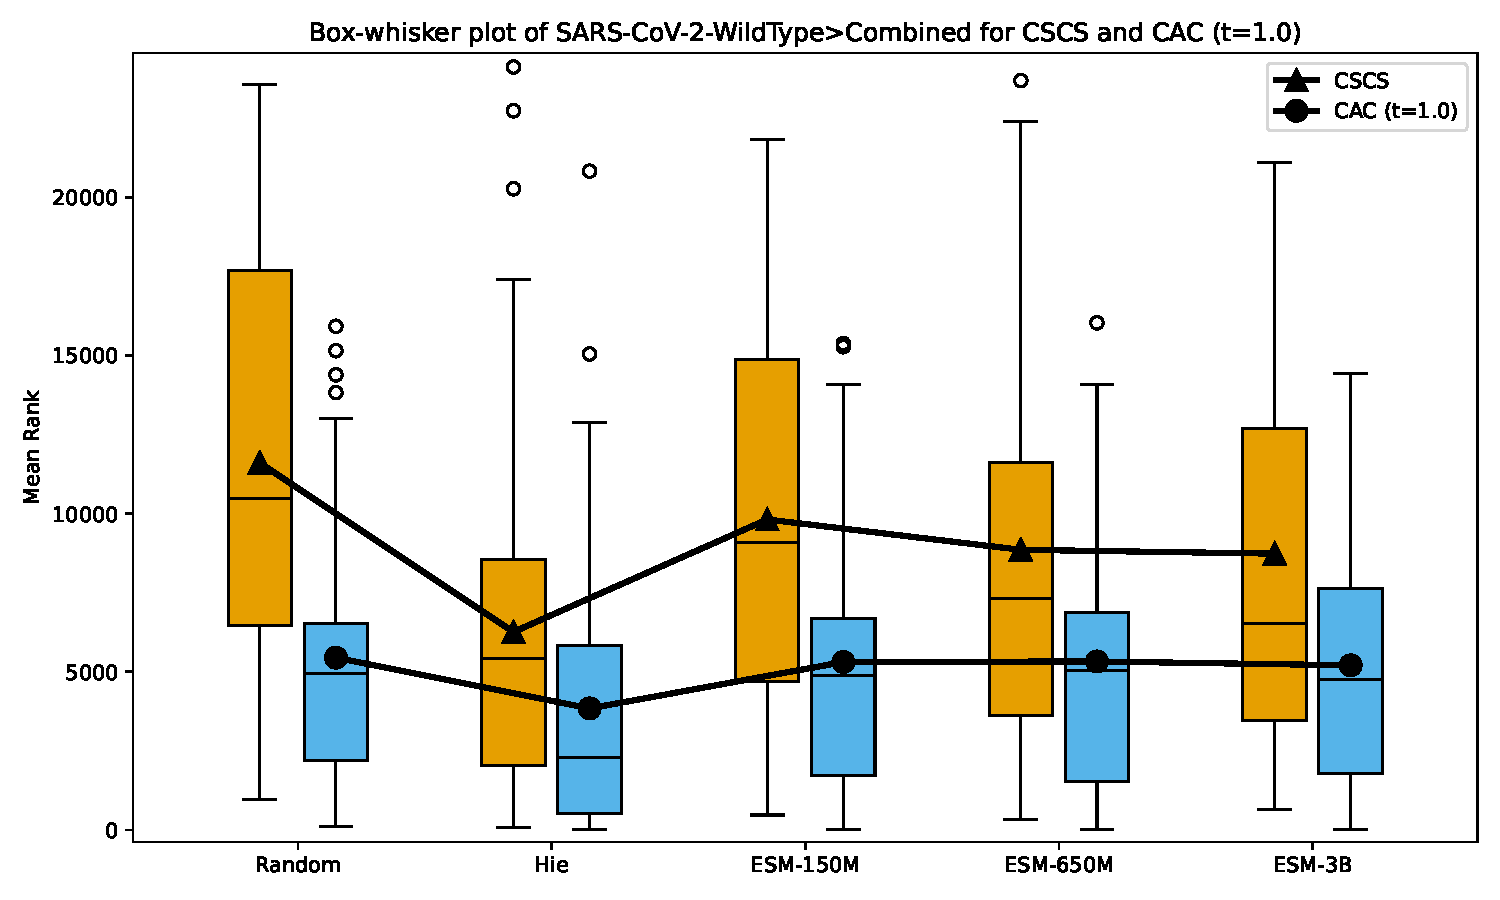
\includegraphics[width=0.48\linewidth]{boxplot-(e=wt2combined)-(t=1.0).pdf}
    \end{tabular}
    \caption{\textbf{Rank distributions across validation sets.}
    Box plots compare CSCS, CAC, CLIMB-only ablation, and random baselines.}
    \label{fig:all-boxplots}
\end{figure}

\begin{table}[htbp]
    \centering
    \caption{\textbf{Representative optimal-weight trajectories.}}
    \begin{tabular}{c|c|c}
        \toprule
        & DMS validation set & Combined validation set \\
        \midrule
        \raisebox{10em}{Hie-BiLSTM} &
        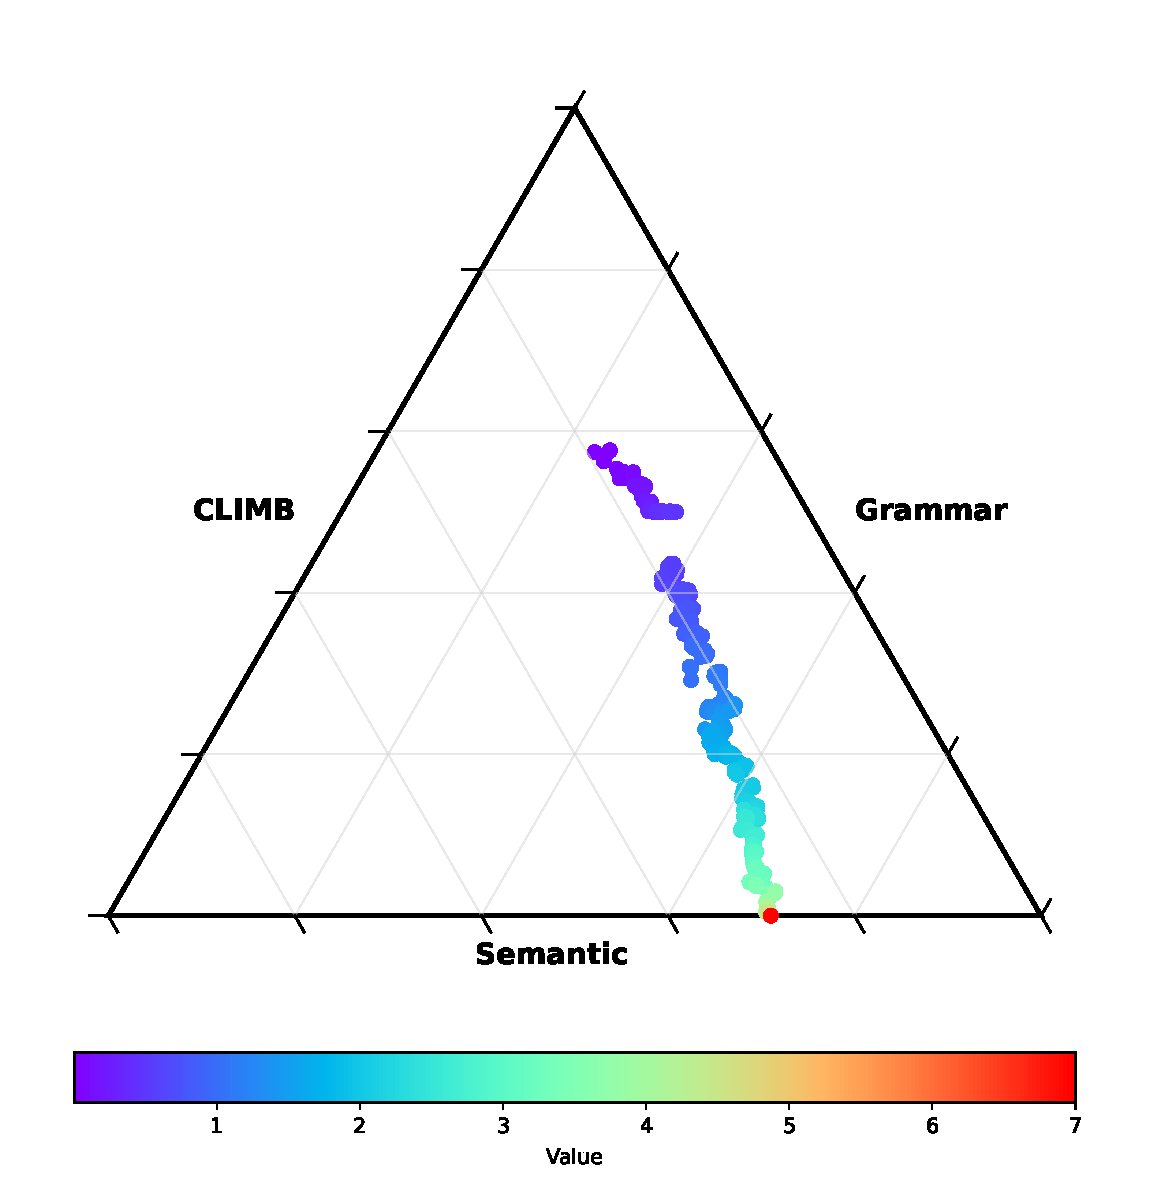
\includegraphics[width=0.4\linewidth]{tri-hie-wt2dms-min.pdf} &
        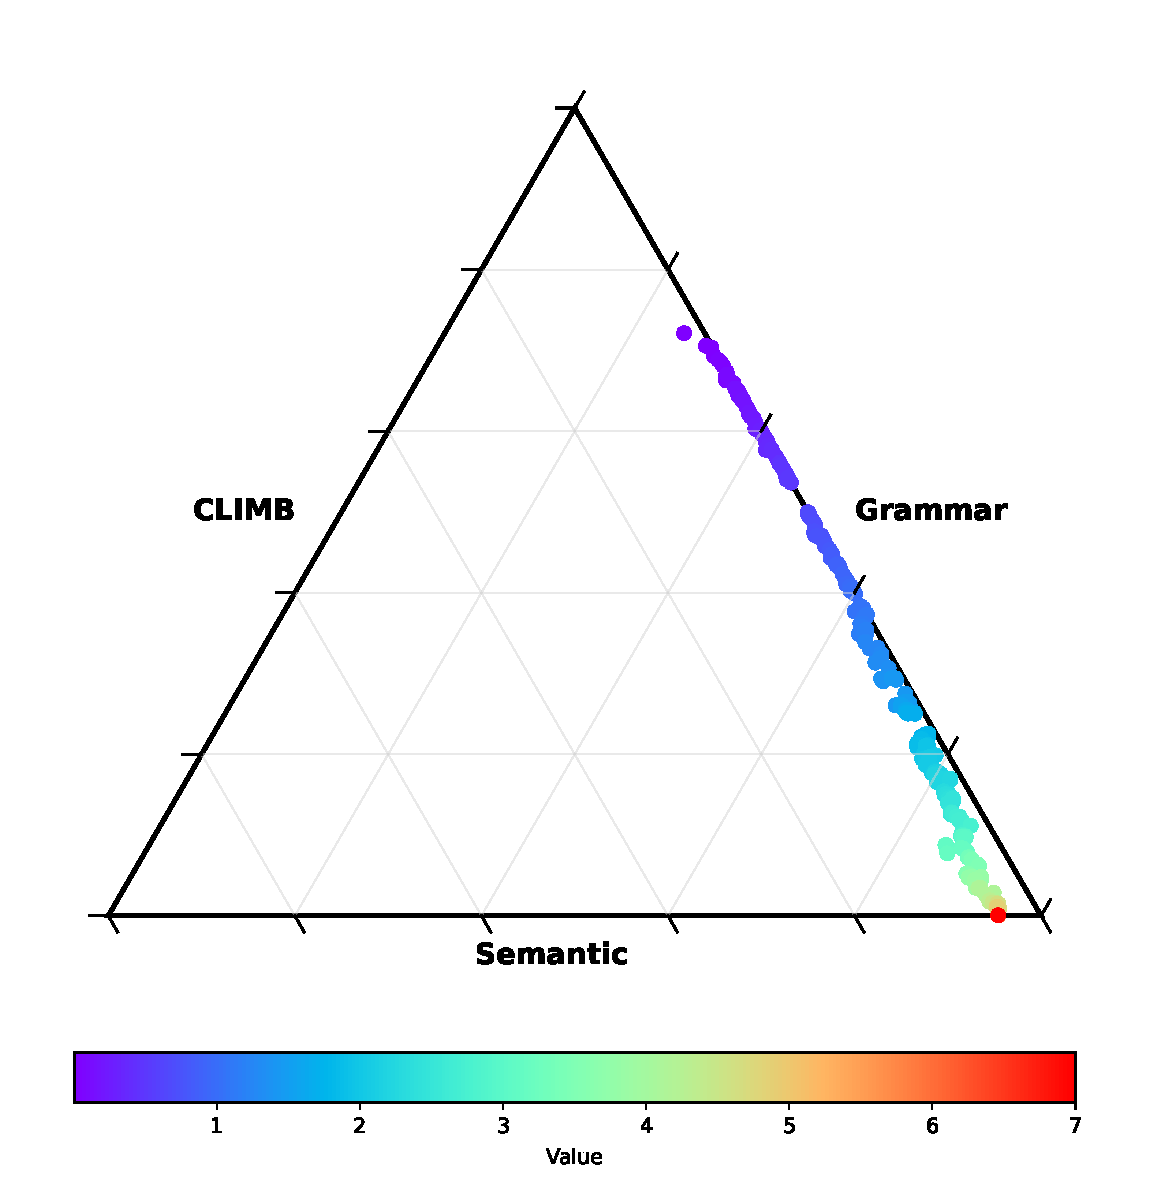
\includegraphics[width=0.4\linewidth]{tri-hie-wt2combined-min.pdf} \\
        \midrule
        \raisebox{10em}{ESM-2-3B} &
        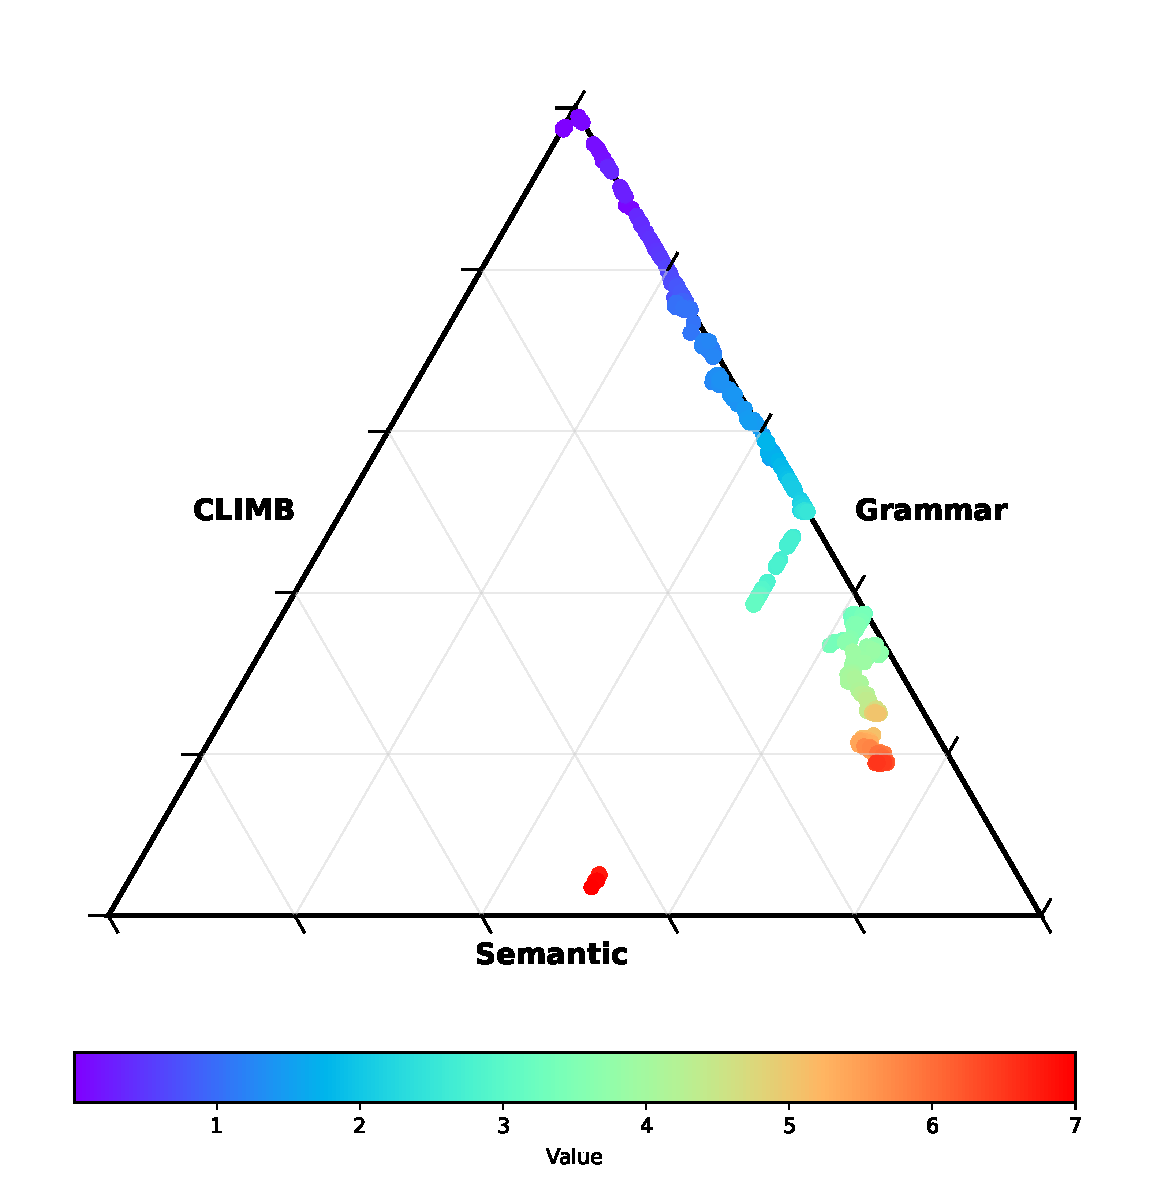
\includegraphics[width=0.4\linewidth]{tri-esm2-3b-wt2dms-min.pdf} &
        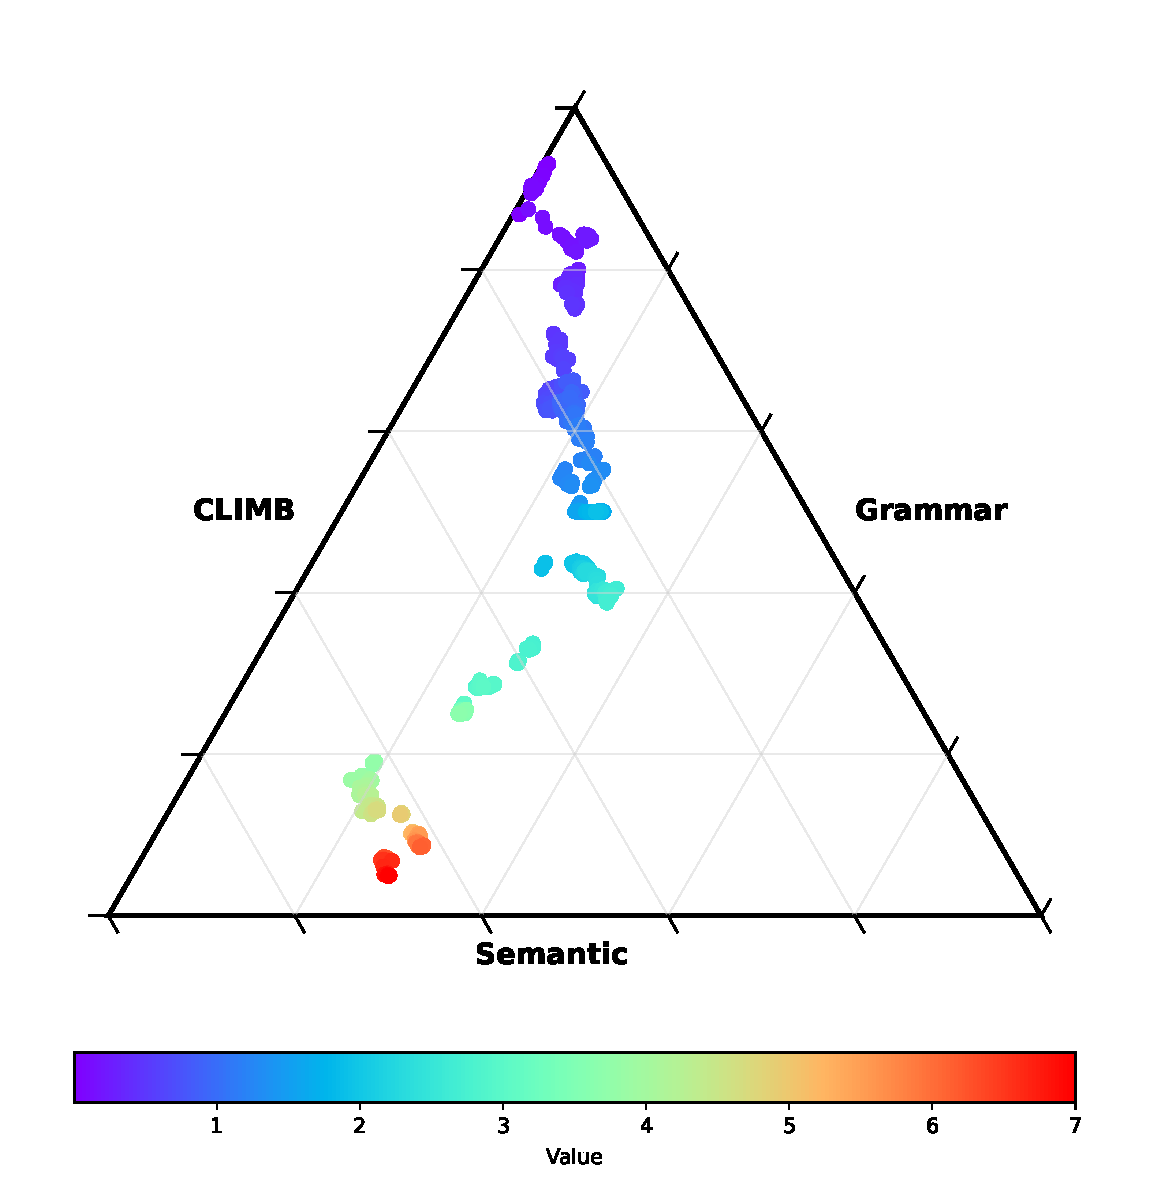
\includegraphics[width=0.4\linewidth]{tri-esm2-3b-wt2combined-min.pdf} \\
        \bottomrule
    \end{tabular}
    \label{tab:weight-trajectories}
\end{table}

\section{Additional landscape analysis}

The PRL manuscript emphasizes the model-process mismatch and the
horizon-dependent crossover. The domain-level Spike landscape analysis from the
long-form manuscript is retained here as diagnostic information. These summaries
should be interpreted as model-behavior diagnostics rather than independent
biological claims.

\begin{table}[htbp]
    \centering
    \caption{\textbf{Domain-resolved average rank shifts for all possible mutations.}
    Negative values indicate promotion by CAC relative to CSCS.}
    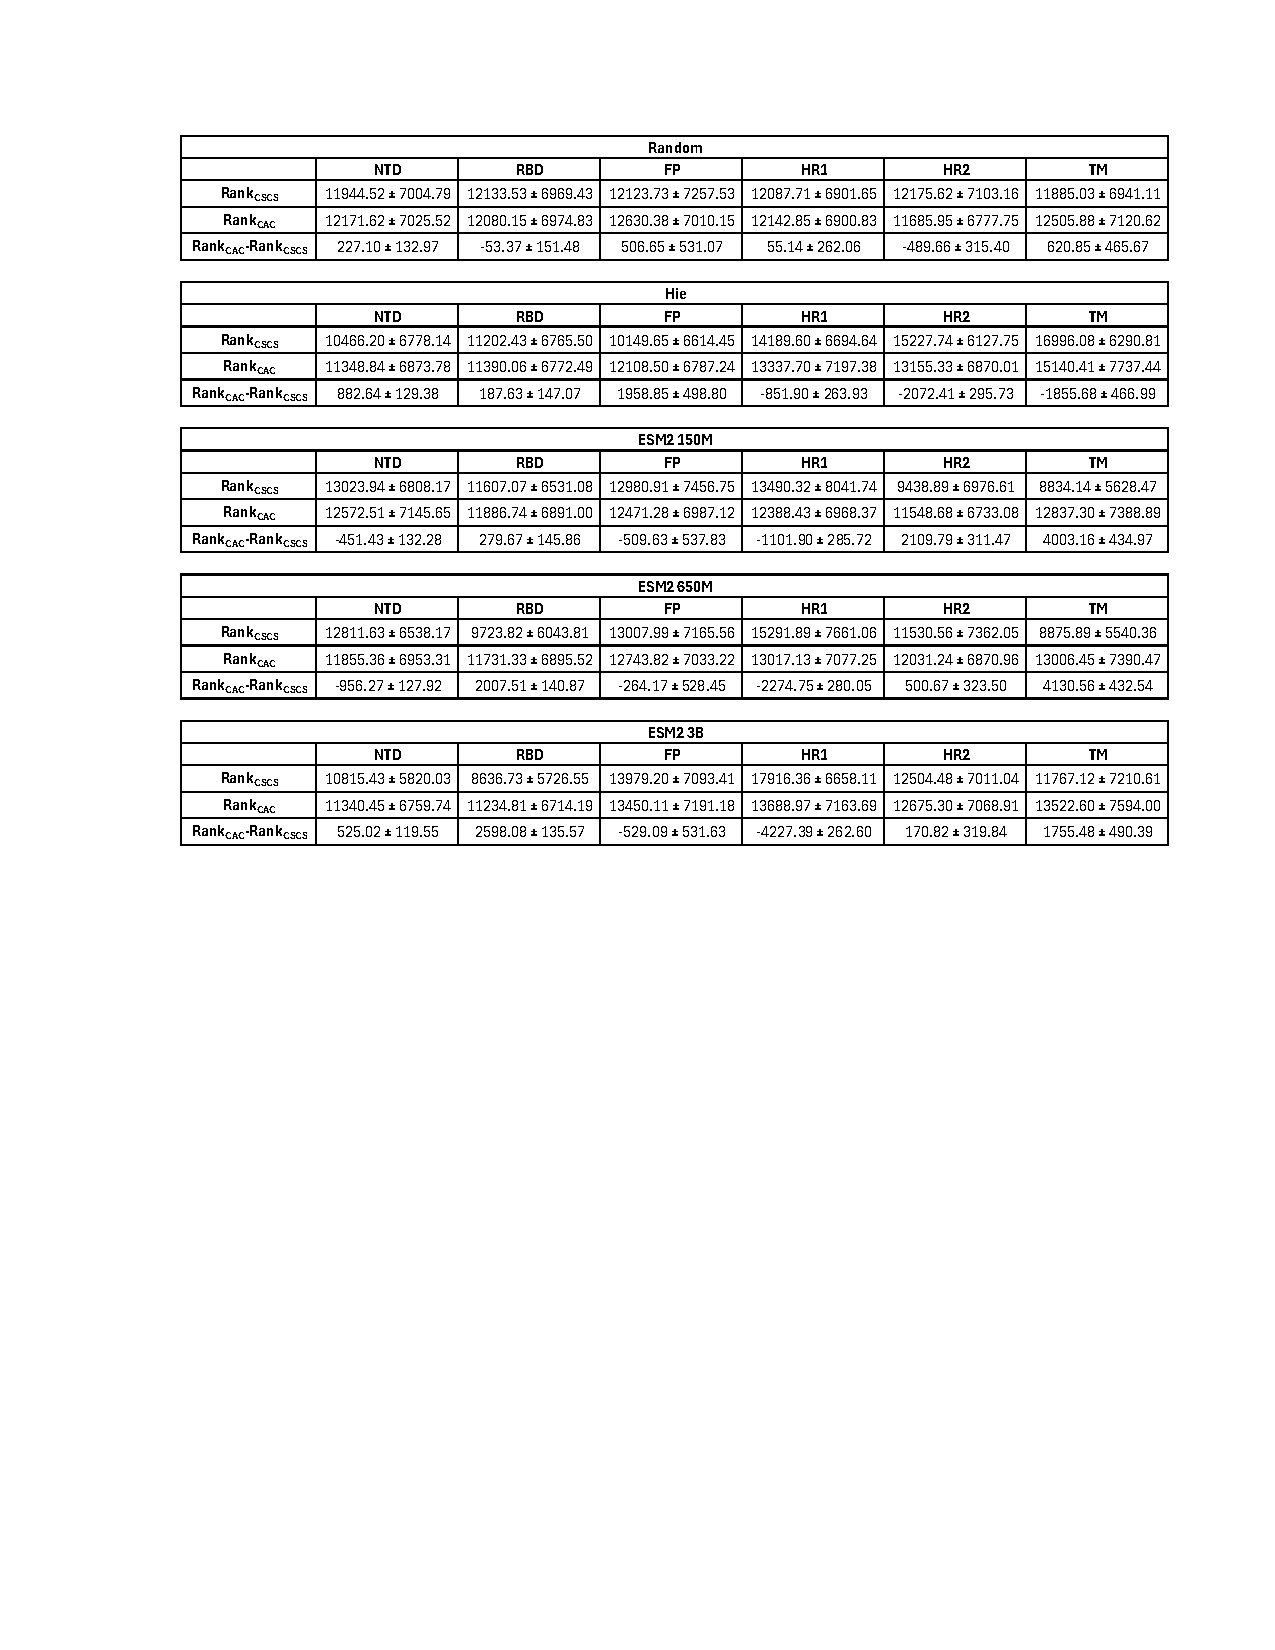
\includegraphics[width=\linewidth]{Supplementary_TableS4.pdf}
    \label{tab:domain-shifts-all}
\end{table}

\begin{table}[htbp]
    \centering
    \caption{\textbf{Domain classification of mutations in the combined validation set.}}
    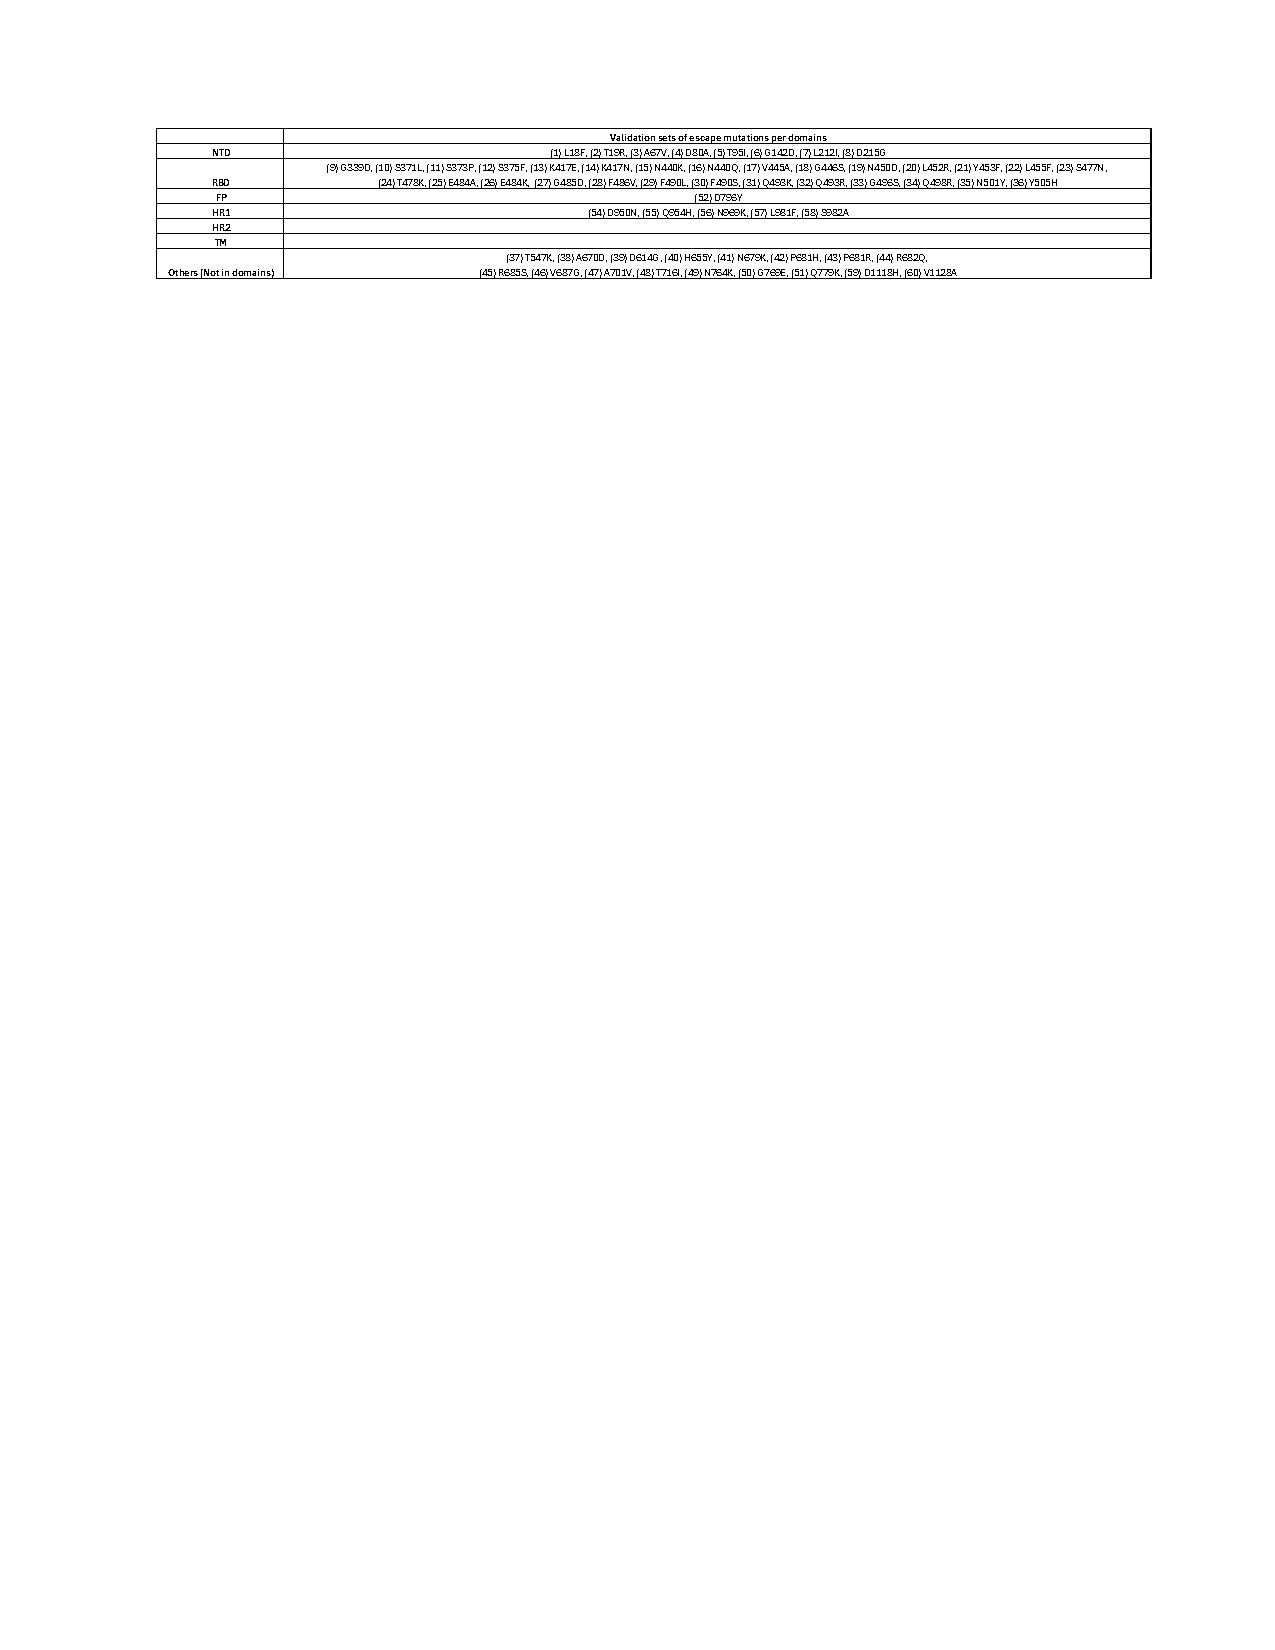
\includegraphics[width=\linewidth]{Supplementary_TableS5.pdf}
    \label{tab:combined-domain-map}
\end{table}

\begin{table}[htbp]
    \centering
    \caption{\textbf{Domain-specific rank changes for the combined validation set.}
    This table focuses only on the 60 known substitutions in the combined set.}
    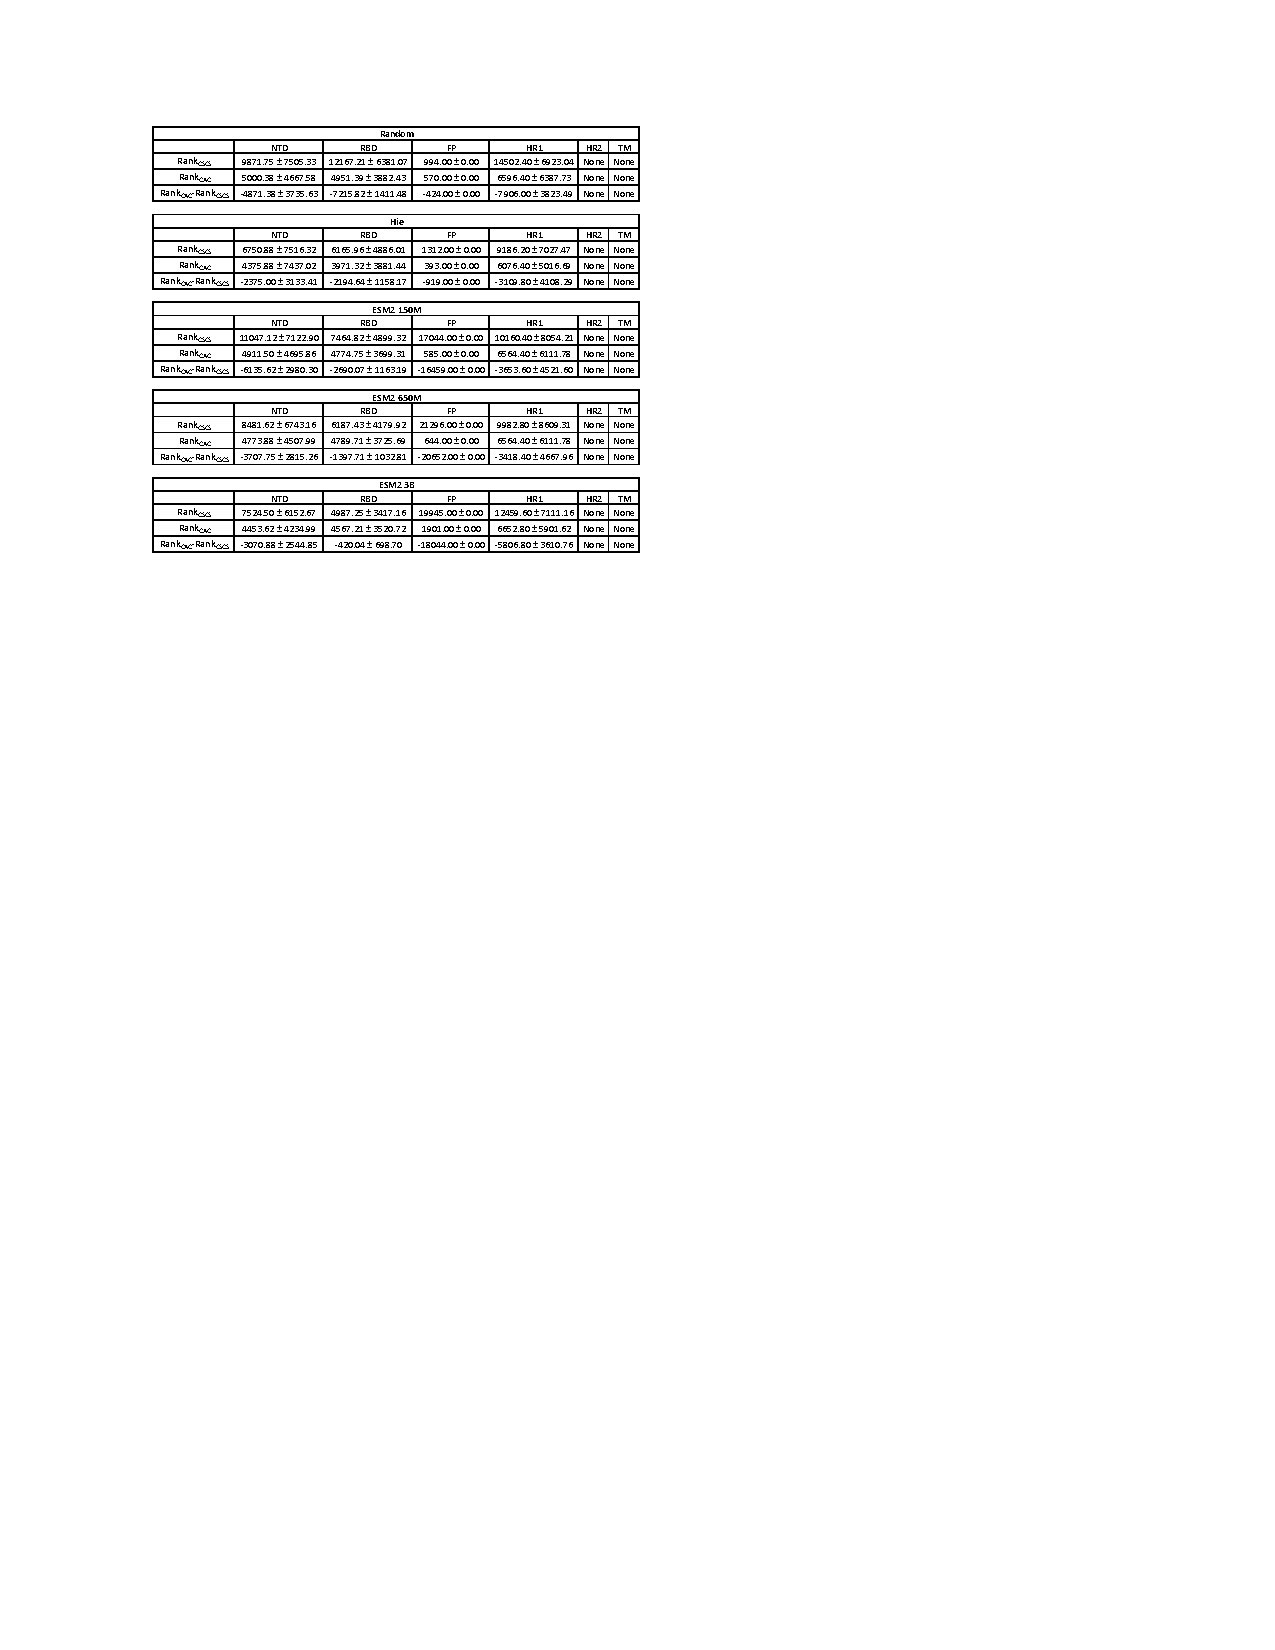
\includegraphics[width=\linewidth]{Supplementary_TableS6.pdf}
    \label{tab:domain-shifts-validation}
\end{table}

\section{Availability and reproducibility}

All source code developed for this study is available at
\url{https://github.com/sos440/climb} and archived on Zenodo at
\url{https://doi.org/10.5281/zenodo.15744443}. The same Zenodo archive contains
the generated CAC scores, CSCS scores, model component scores, and data needed to
reproduce the figures and tables.

The core reproduction workflow is:
\begin{enumerate}[leftmargin=*]
    \item Clone the repository and install dependencies.
\begin{verbatim}
$ git clone https://github.com/sos440/climb
$ cd climb
$ conda create --name climb python=3.10 -y
$ conda activate climb
$ pip install -r requirements.txt
\end{verbatim}
    \item Generate primary scores.
\begin{verbatim}
$ cd viral-analyzer
$ python main.py \
    --escape "SARS-CoV-2-WildType>*" \
    --result "SARS-CoV-2-WildType-*" \
    --scores --seed 42
\end{verbatim}
    \item Optimize component weights.
\begin{verbatim}
$ python main.py \
    --escape "SARS-CoV-2-WildType>*" \
    --result "SARS-CoV-2-WildType-*" \
    --minimizer --seed 42
\end{verbatim}
    \item Run the CLIMB-only ablation.
\begin{verbatim}
$ python main.py \
    --escape "SARS-CoV-2-WildType>*" \
    --result "SARS-CoV-2-WildType-Random" \
    --ablation --seed 42
\end{verbatim}
\end{enumerate}

\FloatBarrier
\printbibliography

\end{document}
